\documentclass[11pt]{book}

\usepackage{makeidx}
\usepackage{hyperref}
\usepackage{graphicx}

\usepackage{tawny}
\lstnewenvironment{tawny}{\lstset{style=tawnystyle}}{}
\lstnewenvironment{clojure}{\lstset{style=clojurestyle}}{}
\lstMakeShortInline[style=clojurestyle]|
%% syntax highlights the same, but does remains commented in Clojure form.
\lstnewenvironment{tawnyexample}{\lstset{style=tawnystyle}}{}

\newcommand{\todo}[1]{\textbf{TODO: #1}}

\usepackage{comment}
\excludecomment{tawnyhidden}

\makeindex

\author{Phillip Lord}

\title{Take Wing: Building Ontologies with Tawny-OWL}


\begin{document}

\maketitle
\tableofcontents

\chapter{Introduction}
\label{cha:introduction}

This book introduces ontology building using the OWL2 ontology language, and
the Tawny-OWL library. Ontologies are a method for representing knowledge,
generally, but not necessarily, about the world around us. It is then possible
to check that the representation is consistent, as well as drawing conclusions
about new knowledge. They are generally used in complex, knowledge-rich areas
of knowledge, including biomedicine.

Many ontology development tools provide a Graphical User Interface, through
which the ontology developer adds the various entities involved in building an
ontology. However, many ontologies contain large and repetitive sections; for
these, ontology development teams often fall back to generating parts of their
ontology programmatically. Tawny-OWL takes a different approach where ontology
development in a domain-specific language (DSL) embedded in a full programming
language. For structurally simple parts of an ontology, the various components
of an ontology can be specified using the default convienient and simple
Tawny-OWL syntax; for structurally complex parts, new syntax and new patterns
can be built, extending the environment as a core part of ontology
development.

This form of programmatic ontology development is still young. At the moment,
we have used it to produce large ontologies that would have been difficult
using any other technique. However, we also hope that we can also support
easier integration of knowledge-rich structures into applications, so that
ontological data structures can be come a standard part of the programmers
toolkit.


\section{Status}
\label{sec:status}

This manual describes Tawny-OWL 2.0. While more Chapters are planned,
it now describes all the key features of this Tawny-OWL environment.

It is hosted at \href{https://phillord.github.io/take-wing/}.



\section{What is an Ontology}
\label{sec:what-an-ontology}

Ontologies are about definitions. It is, perhaps, unsurprising therefore
that amount ontologists there are quite a few debates about what exactly
an ontology is and is not; it is not our intention here to either cover
these arguments, nor to give a comprehensive overview of all the uses of
the word.

What is generally agreed is that ontologies describe a set of entities,
in terms of the relationships between these entities, using any of a
number of different relationships. So, for example, we can describe
entities in terms of their class relationships -- what is true of a
superclass is also true of all subclasses. Or we can describe the
\emph{partonomic} relationships: the finger is part of the hand, which is
part of the foot.

An ontology is also very similar to a taxonomy; however, ontologies
place much greater emphasis on their computational properties. This
makes ontologies much more suitable for driving applications and code,
although this often comes at the cost of human understandability of the
ontology. In this document, all the ontologies we talk about are
represented using specific language, called OWL (the Ontology Web
Language). This has very well-defined computational properties, and
through the document we will explore the implications of these
properties.

We also use the term "ontology" to mean a specific object that you can
manipulate in Tawny-OWL, which is a slightly more constrained use. This is
quite common in many books on programming: we hope that the context should be
clear.

\section{Who this book is for}
\label{sec:who-this-book}

We have two primary audiences for this book. The first is for the ontologist
who is interested in Tawny-OWL as the hub of a new environment for ontology
development. The second is for the programmer who is interested in using the
rich computational representation of a domain that ontologies provide. There
is a risk to having two audiences: that we satisfy neither. To avoid this, the
book is built from a series of chapters, each of which covers a discrete
topic, either more programmatic or more ontological. It should be possible to
read the chapters independently of each other.

This book does not, however, stand alone. While we try to introduce the
background material, we do not intend that, for example, this book will serve
as an introduction to programming either in general, or specifically in
\index{Clojure}Clojure. There are many good resources available for this. With
ontologies, we give more of a background introduction, but again, we assume
that you will be willing to read other material to clarify ontology
development. Our hope is that we introduce the material well enough that you
feel it is worth the time to investigate other resources, and we include
pointers where it seems valuable.






\chapter{A Rapid Walk-Through}
\label{cha:rapid-walk-through}

\section{A Taster}
\label{sec:taster}

We take a rapid walk-through an ontology to demonstrate the capabilities of
Tawny-OWL. As with all the examples in this book, the code in this chapter is
complete, therefore, we need to start with a preamble, defining a namespace
and performing some imports.

\begin{tawny}
(ns take.wing.walk-through
  (:refer-clojure :only [])
  (:use [tawny.owl]
        [tawny.english]
        [tawny.reasoner]))
\end{tawny}

As we discussed in Section~\ref{what_is_an_ontology}, the word ontology has
quite a few different meaning, but here we use it to mean a specific
computational object; so, before, we do anything else, we start a new empty
ontology, which we call |walk_through|; as it happens, we do not need to refer
to this object again because it is now set as the default for the rest of this
chapter. We also take the opportunity to set our choice of reasoner, in this
case HermiT. We will see later how we use this.

\begin{tawny}
(defontology walk_through
  :iri "http://purl.org/ontolink/walk_through")

(reasoner-factory :hermit)
\end{tawny}

Ontologies are all about classes, so we now define two classes one called
|Book| and one called |TakeWing| which is a subclass of |Book|~\footnote{One
  of the joys of ontology development is that the ontology development
  community is rich with arguments about the correct way to model things.
  Even, with relatively simple models it is easy to hit these arguments and,
  in fact, we have done so here already. There is a strong argument to say
  that \lstinline{TakeWing} is actually an instance of \lstinline{Book} rather
  than a subclass, because there is only one of them. Or, that
  \lstinline{TakeWing} is a class because there are many copies of \lstinline{TakeWing}.
  Or, that it's a metaclass, because sometimes it operates like a class and
  sometimes an individual. In this book, we try to touch on these arguments,
  but not get weighed down by them}. Anything that is true of |Book| must also
be true of |TakeWing|.

\begin{tawny}
(defclass Book)

(defclass TakeWing
  :super Book)
\end{tawny}

Of course, this does not tell us much about |TakeWing| as a book. There are
many properties of books, but one of the most informative is the subject of
the book. So, we define a new class of |Subject| and introduce a property
|about| which we use to relate books and subjects~\footnote{Strictly, an
  \emph{object property}, hence the ``o''. We describe these more fully
  later}.

\begin{tawny}
(defclass Subject)

(defoproperty about)
\end{tawny}

Now, we need some subject listings. Of course, there are many of these in
existence already, and Tawny-OWL is fully capable of reusing one of these;
however, for this simple example, it is not necessary, so we define a small
classification of our own. We describe |Bird| and |Ontology| as subclasses of
|Subject| and say that they are different (|:disjoint|) and do not overlap. We
also describe |TawnyOWL| as part of the |Ontology| subject.

\begin{tawny}
(as-subclasses
 Subject
 :disjoint
 (defclass Bird)
 (defclass Ontology))

(defclass TawnyOWL
  :super Ontology)
\end{tawny}

We can now make some basic queries against the statements that we have made to
make sure that they all make sense. So, for example, the |subclasses| function
lists all of the subclasses of |Book|, or we can use the predicate function
|subclass?|. On its own this functionality is enough to build a simple
hierarchy.

\begin{tawny}
(subclasses Book)
;; => #{#[Class 0x660b9d1 "TakeWing"@en]}
(subclass? Book TakeWing)
;;=> true
(subclass? Subject TawnyOWL)
;;=> true
\end{tawny}

However, the functionality of OWL allows much richer statements than this. We
can extend the existing definition of |TakeWing| and state that it is a book
that is about |TawnyOWL| and only about |TawnyOWL|.

\begin{tawny}
(class
 TakeWing
 :super
 (some-only about TawnyOWL))
\end{tawny}

Now, we can build some \emph{defined} classes. We describe an |OntologyBook|
as a |Book| which is about |Ontology|.

\begin{tawny}
(defclass
 OntologyBook
 :equivalent
 (and Book
      (some about Ontology)))
\end{tawny}

There are two critical points about this definition. The first is that we had
said nothing at all about the relationship between this class and |TakeWing|.
We can confirm this by asking about the |subclasses| of |OntologyBook|, and
showing that our ontology knows of no ontology books.

\begin{tawny}
(subclasses OntologyBook)
;;=> #{}
\end{tawny}

However, this is not quite true. The second critical part of the definition,
the use of |:equivalent|. This allows us to use \emph{reasoning} to infer
other subclasses. For this we use the |isubclasses| method instead and find
that |TakeWing| can be infered to be an |OntologyBook|.

\begin{tawny}
(isubclasses OntologyBook)
;; => #{#[Class 0x557ef049 "TakeWing"@en]}
\end{tawny}

We can infer that |TakeWing| is a subclass of |OntologyBook| because we have
said that an ontology book is one about ontologies and that this book is about
Tawny-OWL which is sub-topic of ontologies. Even in this simple example, we
need to put together a number of facts to draw this conclusion.

In this case, though, there is some apparent similarity between the definition
of |OntologyBook| and |TakeWing| -- both of them are look relatively similar,
at least once we substitute |Ontology| for |TawnyOWL| in the definition of
|TakeWing|. Our computational reasoner, however, does not work in this way,
and can draw conclusions even when this similarity does not exist. Consider
this example where we describe books which are not about birds.

\begin{tawny}
(defclass NonBirdBook
  :equivalent
  (and Book
       (not (some about Bird))))

(subclasses NonBirdBook)
;;=> #{}

(isubclasses NonBirdBook)
;; => #{#[Class 0x557ef049 "TakeWing"@en]}
\end{tawny}

Here too, we can classify |TakeWing|. The chain of logic in this case is that
|TakeWing| is about |Ontology|, that |Ontology| is different from |Bird|, and
that, therefore, |TakeWing| is not about |Bird| which makes it a |NonBirdBook|.

This ability to infer new knowledge is the meat and drink of computational
ontologies. They allow a rich description of the environment with a tightly
defined semantics which makes that environment comptutationally accessible.
Here, we have only touched on the expressivity of OWL -- there are many
constructs that we have not shown yet. We have also used this for only for a
small ontology, but as the ontologies grow larger, the value increases.

For existing ontology developers, this will familiar ground. Tawny-OWL,
however, brings something new to other mechanisms for developing ontologies;
that is a fully programmatic environment. As well as the ability to automate
any part of ontology development that we choose, this also brings a rich set
of highly-developed tools that programmers have been developing and using for
many years to develop software in a repeatable, scalable and
highly-collaborative way. It is this which we explore next.


\section{Environment}
\label{sec:environment}

Tawny-OWL takes a different approach to other ontology development
environments. It is not an application, it is just a programmatic
library\footnote{Sort of. In other environments, we have argued that Tawny-OWL
  is an textual application rather than a programmatic library. In reality, it
is a bit of both: it is a library which is designed with development rather
than manipulation of ontologies as its primary purpose. For the latter, we
would have done things rather differently.}. This has a
key advantage over a more traditional ontology editor; rather than providing
a complete environment, Tawny-OWL just recasts ontology development as a form
of software development and borrows its entire environment from software
development. This means we can reuse the software engineering environment; our
experience is that the richness and maturity of software development tools far
outweights any loss of specificity to ontology development.

Our hope is that for structurally simple ontologies, Tawny-OWL should be
usable by non-programmers, with a simple and straight-forward syntax. In this
section, we introduce the core technology and the basic environment that is
needed to make effective use of Tawny-OWL, as well as some optional extras.


\subsection{The OWL API}
\label{sec:owl-api}

Tawny-OWL is built using the \url{http://owlapi.sourceforge.net/[OWL} API].
This library is a comprehensive tool for generating, transforming and using
OWL Ontologies. It is widely used, and is the basis for the Protege 4
editor\cite{greycite2912}. Being based on this library, Tawny-OWL is reliable
and standard-compliant (or at least as reliable and standard-compliant as
Protege!). It is also easy to integrate directly with other tools written
using the OWL API, include Protege.

\subsection{Clojure}
\label{sec:clojure}

Tawny-OWL is a programmatic library build on top of the Clojure
language. Tawny-OWL takes many things from Clojure. These include:

\begin{itemize}
\item the basic syntax with parentheses and with \texttt{:keywords}
\item the ability to effectively add new syntax
\item the ability to extend Tawny-OWL with patterns
\item integration with other data sources
\item the test environment
\item the build, dependency and deployment tools
\end{itemize}

In addition, most of the tools and environment that Tawny-OWL use to
enable development were built for Clojure and are used directly with
little or no additions. These include:

\begin{itemize}
\item IDEs or editors used for writing Clojure
\item the leiningen build tool
\end{itemize}

Tawny-OWL inherits a line-orientated syntax which means that it works
well with tools written for any programming language; most notable
amoung these are version control systems which enable highly
collaborative working on ontologies.

Clojure is treated as a programmatic library -- the user never starts or
runs Clojure, and there is no \texttt{clojure} command. Rather confusingly,
this role is fulilled by Leiningen, which is the next item on the list.

\subsection{Leiningen}
\label{sec:leiningen}

\url{http://www.leiningen.org[Leiningen}] is a tool for working with Clojure
projects. Given a directory structure, and some source code leiningen
will perform many project tasks including checking, testing, releasing
and deploying the project. In addition to these, it has two critical
functions that every Tawny-OWL project will use: first, it manages
dependencies, which means it will download both Tawny-OWL and Clojure;
second, it starts a REPL which is the principle means by which the user
will directly or indirectly interact with Tawny-OWL.

\subsection{REPL}
\label{sec:repl}

Clojure provides a REPL -- Read-Eval-Print-Loop. This is the same things
as a shell, or command line. For instance, we can the following into a
Clojure REPL, and it will print the return value, or 2 in this case.


\begin{tawny}
;; returns 2
(+ 1 1)
\end{tawny}

The most usual way to start a REPL is to use leiningen, which then sets
up the appropriate libraries for the local project. For example,
\texttt{lein repl} in the source code for this document, loads a REPL with
Tawny-OWL pre-loaded.

In practice, most people use the REPL indirectly through their IDE.

\subsection{IDE or Editor}
\label{sec:ide-or-editor}

Clojure is supported by a wide variety of editors, which in turn means
that they can be used for Tawny-OWL. The choice of an editor is a very
personal one (I use Emacs), but in practice any good editor will work.

The editor has two main roles. Firstly, as the name suggests it provides
a rich environment for writing Tawny-OWL commands. Secondly, the IDE
will start and interact with a REPL for you. This allows you to add or
remove new classes and other entities to an ontology interactively.
Tawny-OWL has been designed to take advantage of an IDE environment; in
most cases, for example, auto-completion will happen for you.

\subsection{Testing}
\label{sec:testing}

Tawny-OWL can use any of the testing enviroments that come with Clojure,
including |clojure.test| which is the most basic environment provided with
Clojure. This integrates well with both leiningen or an IDE both of which will
run tests for you and report on test cases.

\subsection{Version Control and Collaboration}
\label{sec:vers-contr-coll}

Most ontologies are developed by many people, so some form of collaboration
support is needed. In general, with Tawny-OWL we achieve this in the same way
that programmers do; rather than providing a collaborative environment where
multiple people can edit the environment at the same time, we use version
control where different developers use slightly different versions of the
ontology, and then merge them together at the end. This works well with
Tawny-OWL as it has an attractive, line-orientated syntax. The various version
control tools can scale easily to thousands of developers which is well in
excess of most ontology projects. For this purpose, we use |git|.

\subsection{Continuous Integration}
\label{sec:cont-integr}

An ontology can be \emph{continuously integrated} with both other ontologies
that it depends on, and with the software environment which uses it. Unlike
other ontology continuous integration systems, Tawny-OWL is just a library --
so anything that works with Clojure (or more abstractly a Java Virtual
Machine) will also work with Tawny-OWL.

\section{Recap}
\label{sec:recap}

In this Chapter, we have built a small basic ontology which non-the-less shows
the computational power of OWL ontologies, while surveying the advantages that
Tawny-OWL brings as a development environment for ontologies.




\chapter{An Introduction to OWL}

In Section\ref{sec:what-an-ontology}, we briefly touched on the issue
of what is an ontology and noted that it's not easy. In this section,
we will take a more pragmatic view point and describe OWL and its
notion of an ontology.

OWL2 is the second version of the Ontology Web Language; it is a W3C
recommendation\footnote{W3C is the body that would define standards
  for the Web, if it makes standards. Except that it does not; it just
releases recommendations.}. As you might expect, this means that it
embeds well with other W3C standards -- it can be serialized as XML or
RDF, and it makes quite intensive use of URLs.

It also builds on many years of Computing research; underneath each of
the statements that we can make in OWL is a mapping to a piece of
formal maths which gives a tightly defined \emph{semantics}. We will
only touch of this semantics lightly in this document\footnote{Mostly
  because if I touched on it more heavily, I'd probably get it wrong};
the key point is that this specification makes it possible to build
software around OWL and have it come to a clearly defined conclusions.

Using the statements in OWL we can build models of the world. That is
we can describe the real world around us using statements in OWL; as a
result, we can use these underlying semantics of OWL to draw
conclusions about these models. If we do this right, these conclusions
should also be true of the real world as well.

There are a number of different ways that we could build models, but
OWL does this with three entities: individuals, classes and
properties. In addition, to enable OWL ontologies to describe the real
world, it also has two further entities: identifiers and annotations.


\section{Individuals}
\label{sec:individuals}

At heart, OWL ontologies describe a set of individuals. In the real
world, these would be the things that we want to describe. Looking
around me now, I can see a large number of these things: a computer
screen (obviously); a keyboard; assorted other pieces of computing
detritus; a guitar; a door; and, finally, somewhat incongruously, a
toilet seat. Individuals in OWL can also describe more abstract things
such as the image on my screen, the process of me typing and so forth.

Sometimes, individuals are also called instances; we do not use this
term here, because it causes confusion with people who come
Object-Oriented programming background where it has a related but
subtly different meaning\footnote{Like ``object'' which also has an
  ontological meaning.}.

In OWL ontologies, individuals also have a name or an
identifier\footnote{Although, some individuals are anonymous. We will
  discuss more on the form of identifiers later.}. Actually, they can
any number of names and, perhaps, unintuitively, OWL will not assume
that they have an unique name; so, unless you tell it explicitly, OWL
will not know whether two different identifiers describe two different
individuals with one name each, or one individual with two names.

\section{Properties}
\label{sec:properties-1}

Individuals can have relations between them. In OWL, these are called
properties\footnote{Roughly equivalent to properties or attributes in
  OO terminology}. So, the |I| and |typing| on my |Keyboard|. In OWL
properties are \emph{binary} -- that is they only describe a
relationship between two individuals\footnote{This is less restrictive
  than it sounds.}. Properties in OWL have a number of
characteristics, which we will describe later.

It is also possible to use properties to describe a relationship
between an individual and something \emph{concrete} -- such as a
numeric value or a string.

\section{Classes}
\label{sec:classes}

Classes in OWL are \emph{sets} on individuals. All the individuals in
a class will share some of the same characteristics. Classes have
relationships between themselves which turn them into a hierarchy. So,
both my |Trackball|, |Keyboard| and |Monitor| are subclasses of
|Peripherals|. In OWL, the meaning of the subclass relationship is
quite specific -- if |A| is a subclass of |B|, then all individuals of
class |A| are also individuals of class |B|.

For people coming from an programming background, this looks very like
object-orientation (OO) and its notion of instances, classes and
subclasses. But there is subtle, but important difference. In OO,
instances are explicitly stated to be part of a class, and inherit
properties from this class. In OWL, it is the other way around:
individuals have properties, and then properties that they have define
the classes that they are in. We can see this in
Section~\ref{sec:taster}, where we can \emph{infer} that |TakeWing| is
an |OntologyBook|.

\section{Identifiers}

To make all of the logical entities in OWL useful, we need
\emph{identifiers} which allows us to refer to them. Again, most
programming languages have this sort of capability: variable names,
class names and so forth. OWL is rather different here and shows its
web heritage; it uses IRIs for identifiers\footnote{IRIs are not the
  same thing as URIs, which are not the same thing as URLs. But the
  differences between them are relative unimportant here.}.

Identifiers in OWL, therefore, are effectively universal; a class in
one ontology can unambiguously refer to a class in another. More over,
it can use and share identifiers described and defined in all the
other web technologies.

\tawny maps these identifiers on to its own which inherits from its
base language of Clojure; this largely stems from the requirements for
identifiers which are easy to type and use.


\section{Annotations}

Those who are interested in the underlying semantics of OWL often
describe annotations are \emph{extra-logically}. This rather
downgrades their importance; it is annotations that allow the
underlying logic to relate to the real world around. The underlying
logic of OWL may provides predictable behaviour, but is the
annotations which provide all the utility of an OWL ontology, by
relating to the real world and to the user.

OWL allows annotations on pretty much anything. Classes, individuals
and properties can all have annotations; the axioms that assert these
entities can have annotations; annotations can have annotations; it is
even possible to use annotations to provide descriptions of why
annotations have annotations. It is entirely possible that the
designers of OWL got a little carried away with annotations, \tawny
supports the many different forms of annotation anyway.

\chapter{Getting Started}

In this section, we will build the most ontology and start to show the
basic capabilities of Tawny-OWL.

As described in \label{/the/environment-the-environment}, Tawny-OWL can be
used with several different toolchains. In this section, we will run
through the building a very simple ontology. There is an section describing
how to achieve each of these steps with specific tool chains.

\subsection{Installing Leiningen}

To build an ontology, we need a build tool, for which we will use
\url{https://leiningen.org}{leiningen}. This is a command line
application and is simple to install following the instructions on
their website.

Installing leiningen is the only manual step involved. It is leiningen
that is responsible for everything else; it downloads Tawny-OWL and
all of its dependencies for you.

\subsection{Creating a New Project}

Now, we will create a new project. Tawny-OWL makes this easy with a
pre-defined template.

\begin{verbatim}
lein new ontology helloworld
\end{verbatim}

This will create a new directory called |helloworld|. If we change
into this directory, we find that this has created a number of
directories and files.

Before we look in more detail at these files, let start by generating
an ontology file. Simply type:

\begin{verbatim}
lein run
\end{verbatim}

You should see that a new file has been created called
\verb|helloworld.omn| which contains a very simple ontology with a
single class called |HelloWorld|.

\subsection{Editing Our Ontology}

Tawny-OWL provides a fully programmatic development environment for
ontologies; as such, it is possible to change or update an ontology
with an editor or any IDE. In this section, we will use a simple,
web-based editor that integrates tightly with leiningen.

To use this try:

\begin{verbatim}
lein with-profile light nightlight
\end{verbatim}

This should return something like:

\begin{verbatim}
Started Nightlight on http://localhost:4000
\end{verbatim}

Open this address in a web-browser and you should now be able to see
the editor. This in turn will enable you to look at the Tawny-OWL files.

First, we consider the file |helloworld.clj|; this looks like so:

\lstinputlisting[style=tawnystyle]{../new-project/helloworld/src/helloworld/helloworld.clj}

Breaking this down. We first start with by introducing the namespace
and |use|ing Tawny-OWL. These identical statements appear at the
beginning of every Tawny-OWL file: the namespace introduced must match
the file name.

Next, we create a new ontology called |helloworld|, with a single
class also called (somewhat repetitively), |HelloWorld|. Tawny-OWL is
case-sensitive, so these two things are independent from each other.

The second file, |core.clj| is more programmatic in nature. It
|require|s |helloworld|, and then defines a function called |-main|
which saves the ontology.

\lstinputlisting[style=tawnystyle]{../new-project/helloworld/src/helloworld/core.clj}

The practical upshot of this all taken together is that typing

\begin{verbatim}
lein run
\end{verbatim}

at the command line will result in a new file (called
|helloworld.omn|) with an ontology in OWL Manchester Notation (OMN).

\subsection{Summary}

In this section, we have outlined the basic tasks that are needed to
build ontologies with Tawny-OWL: creating a project, creating an
ontology, creating some entities. We have also started to show how to
use and query over them. In the next section, we will build this
ontology in full, using it to demonstrate many parts of Tawny-OWL and
OWL ontologies in general.



\chapter{The Pizza Ontology}
\label{cha:pizza-ontology}

\section{Introduction}
\label{sec:introduction}

In this section, we will create a Pizza ontology; we choose pizzas because
they are simple, well-understood and compositional (see
\href{http://robertdavidstevens.wordpress.com/2010/01/22/why-the-pizza-ontology-tutorial/}{here}
for more).

As we described in a previous Chapter~\ref{cha:an-introduction-owl},
we consider the different types of entities present in an OWL
ontology. The most (and least!) important of these are
\emph{individuals}. We say that these are the most important because
it is these individuals that are described and constrained by the
other objects. We say that they are the least important because, in
practice, many ontologies do not explicitly describe any individuals
at all.

If this seems perverse, consider a menu in a pizza shop. We might see
an item saying "Margherita\ldots{}.£5.50". The menu makes no
statements at all about an individual pizza. It is saying that any
margherita pizza produced in this resturant is going to (or already
has) cost £5.50. From the menu, we have no idea how many margherita
pizzas have been produced or have been consumed. But, menu is still
useful. The menu is comprehensive, tells you something about all the
pizzas that exist (at least in one resturant) and the different types
of pizza. This is different to the bill, which describes individuals
-- the pizzas that have actually been provided, how many pizza and how
much they all cost.  In ontological terms, the menu describes the
\textbf{classes}, the bill describes individuals \footnote{The analogy
  between a pizza menu and an ontology is not perfect. With pizza,
  people are generally happy with the classes (i.e. the menu) and
  start arguing once about the individuals (i.e. the bill); with
  ontologies it tends to be the other way around}. OWL Ontologies
built with Tawny-OWL \emph{can} describe either or both of these
entities but in most cases focus on classes.

\section{Creating the Skeleton}

As we discussed in Section~\ref{sec:creating-new-project}, it is
possible to use leiningen to create a new ontology project. We will do
this now:

\begin{verbatim}
lein new ontology take-wing-pizza
\end{verbatim}

This will create a directory called |take-wing-pizza|\footnote{The
  name of this directory is not functional important and be changed at
will}. We can now edit the files in this directory, starting with
|take/wing/pizza.clj| using either nightlight as described in
Section~\ref{sec:editing-our-ontology}, or any other IDE.


\section{Preamble}
\label{sec:preamble}

In Chapter~\ref{cha:rapid-walk-through}, we showed the standard
template for a Tawny-OWL file; and indeed, leiningen has created a
pizza themed version for us.

\begin{tawnyexample}
(ns take.wing.pizza
  (:require [tawny.owl :refer :all]))
\end{tawnyexample}

It is not absolutely critial to understand these statements, but they
are simple enough and worth explaining now, even though they will
become much more relevant and start to exploit the underlying
programming language of Tawny-OWL, that is Clojure.

Statements in Clojure are also known as ``forms''. Pretty much all
Clojure forms have the same structure; that is they are delimited by
|(| and |)|. Forms are usually named after the first letters that
appear in them, which is the name of the function they will call; so
in this case, we have a |ns| or ``namespace'' form. Forms can be
nested. The |:require| form is an example of this. In this case, the
|:require| says simply to make the Tawny-OWL functions available for
use. The colon in |:require| means that this is a
\emph{keyword}. Tawny-OWL uses these in many places to define
parameters, as we see next. Before we go any further, let's make this
slightly more complex:

\begin{tawny}
(ns take.wing.pizza
  (:require [tawny.owl :refer :all]
            [tawny.reasoner :as r]))
\end{tawny}

We will see the importance of |tawny.reasoner| later. Next, we have a
|defontology| form which looks like this:

\begin{tawnyexample}
(defontology take-wing-pizza
  :iri "http://example.com/take-wing-pizza")
\end{tawnyexample}

The name of the function |defontology| tells us something useful; as
well as creating an ontology, we are defining a name which we can use
to refer to the ontology. The name is |take-wing-pizza| which comes
next. Finally, we define some parameters -- in this case, the IRI. All
OWL ontologies require IRIs (strictly the Ontology IRI) by which they
can be refered\footnote{In Tawny-OWL, this requirement is weakened --
  if you do not put an IRI, Tawny-OWL invents one for you. This is
  okay if you are experiments, but should be changed when you publish
  an ontology.}. Here, we invent one in the |example.com| domain. You
should change this to an IRI you control. In this case, we use one
from |purl.org|.

\begin{tawny}
(defontology take-wing-pizza
  :iri "http://purl.org/ontolink/take-wing/pizza")
\end{tawny}

The semantics of this statement are quite interesting. If we had created
a new database, by default, the database would be considered to be empty
-- that is there would be no individuals in it. With an ontology, the
opposite is true. By default, we assume that there could be any number
of individuals. As of yet, we just have not said anything about these
individuals.

\section{Defining Classes}
\label{sec:defining-classes}

Next, we declare two classes. A class is a set of individuals with
shared characteristics. The basic template creates an entirely useless
|HelloWorld| task for us like so:

\begin{tawnyexample}
(defclass HelloWorld)
\end{tawnyexample}

This follows the same syntax as all forms with |(| and |)|, and
follows the convention of |defontology| -- a class object is created
as well as a name |HelloWorld| which we can use to refer to that
object. In this case, we do not add any arguments nor do we need
to. If you are using nightlight, it should look like this:

\begin{figure}
  \centering
  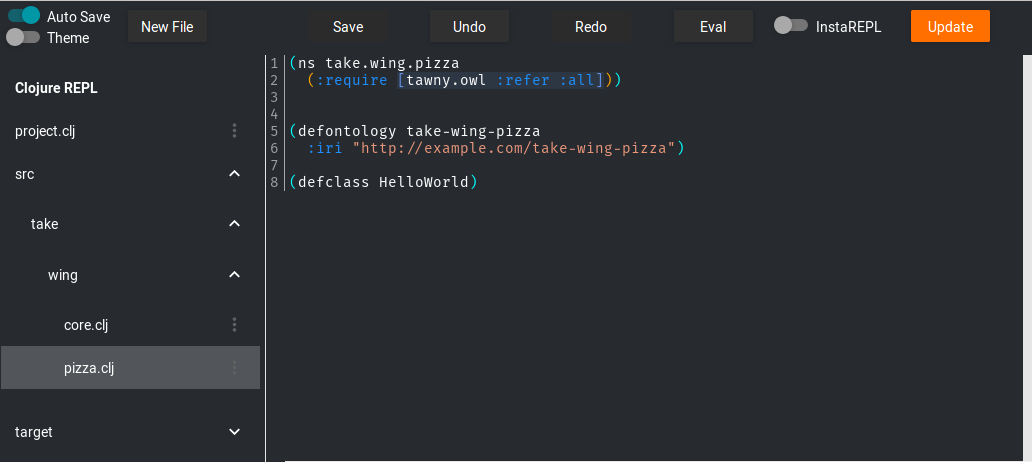
\includegraphics[width=\textwidth]{images/night-pizza.png}
  \caption{A new pizza ontology}
  \label{fig:nightlight-pizza}
\end{figure}

It is possible to run, or evaluate, Tawny-OWL files as well. To see
this in nightlight, simply select ``Insta-REPL'' on the top-right.

\begin{figure}
  \centering
  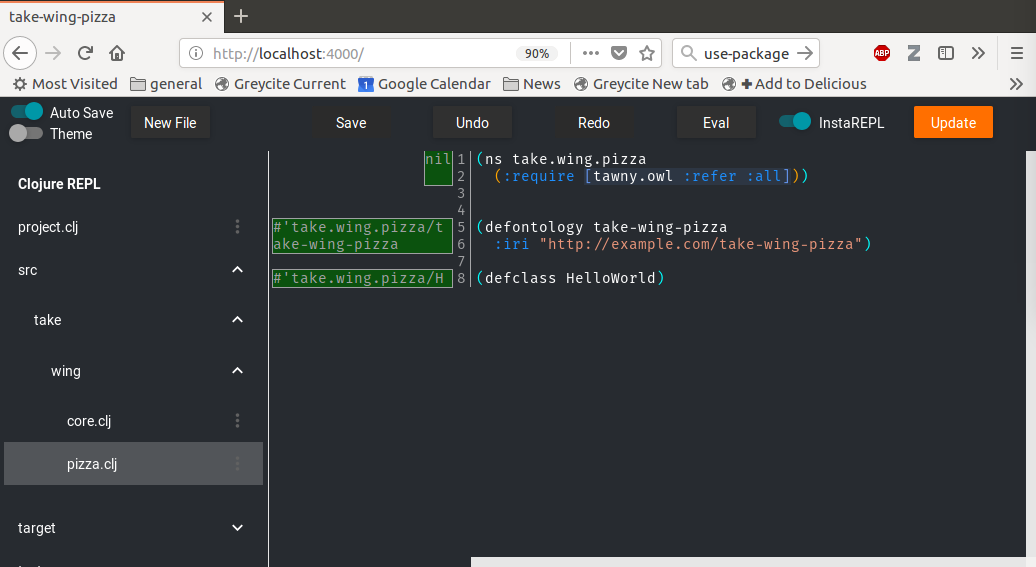
\includegraphics[width=\textwidth]{images/night-instarepl.png}
  \caption{The Insta-REPL}
  \label{fig:nightlight-pizza}
\end{figure}

On the left, we can see the results of this evaluation. The actual
values are not that useful in Tawny-OWL, but the that they are green
shows that they are valid.

Clearly, as this is supposed to be an ontology of pizza rather than
classic computer programs, we will need to change this. So, first we
replace |HelloWorld| with |Pizza| and add a new class called
|PizzaComponent|.  As with our |defontology| form, have a |def| form;
however, in this case, we do not use any arguments. The semantics of
these two statements are that, there is a class called |Pizza| and
another called |PizzaComponent| which individuals may be members of.
However, we know nothing at all about the relationship between an
individual |Pizza| and an individual |PizzaComponent|\footnote{In this
  ontology, we use a naming scheme using CamelCase, upper case names
  for classes and, later, lower case properties. As with many parts of
  ontology development, opinions differ as to whether this is
  good. With Tawny-OWL it has the fortuitous advantage that it syntax
  highlights nicely, because it looks like Java class names.}.

\begin{tawnyexample}
(defclass Pizza)
(defclass PizzaComponent)
\end{tawnyexample}

To build an accurate ontology, we may wish to describe this relationship
further. We might ask the question, can an individual be both a |Pizza|
and a |PizzaComponent| at the same time. The answer to this is no, but
currently our ontology does not state this. In OWL terminology, we wish
to say that these two classes are \emph{disjoint}. We can achieve this by
adding an |as-disjoint| statement.

\begin{tawnyexample}
(as-disjoint Pizza PizzaComponent)
\end{tawnyexample}

This works well, but is a little duplicative. If we add a new class
which we wish to also be disjoint, it must be added in two places.
Instead, it is possible to do both at once. This has the advantage of
grouping the two classes together in the file, as well as semantically,
which should make the source more future-proof; should we need new
classes, we will automatically become disjoint as required.

\begin{tawnyexample}
(as-disjoint
 (defclass Pizza)
 (defclass PizzaComponent))
\end{tawnyexample}

If you are using Nightlight, you may find it a little hard to edit
your file to achieve this as Nightlight uses
\href{http://shaunlebron.github.io/parinfer/}{parinfer}. This puts the
parentheses in place for you. To make this statement, type
|as-disjoint| before the other two forms:

\begin{tawnyexample}
(as-disjoint)
(defclass Pizza)
(defclass PizzaComponent)
\end{tawnyexample}

Now, add two spaces in front of \lstinline|defclass Pizza)| and then
\lstinline|(defclass PizzaComponent)|. The parentheses should take care of themselves.

\begin{tawny}
(as-disjoint
 (defclass Pizza
   :label "Pizza"
   :comment "A type of prepared food, originating from Italy, consisting of a
flatbread with any of a large variety of other foods on top.")
 (defclass PizzaComponent
   :label "Pizza Component"
   :comment "Food that is part of a pizza."))
\end{tawny}

The semantics of these statements are that our ontology may have any
number of individuals, some of which may be |Pizza|, some of which may
be |PizzaComponent|, but none of which can be both |Pizza| and
|PizzaComponent| at the same time. Before we added the |as-disjoints|
statement, we would have assumed that it was possible to be both. We
also add to this two \emph{annotations} that can be used to provide
more contextualized information about the pizza -- in this case a
label and a comment.

As well as describing that two classes are different, we may also wish
to describe that they are closely related, or that they are
\emph{subclasses}. Where one class is a subclass of another, we are saying
that everything that is true of the superclass is also true of the
subclass. Or, in terms of individuals, that every individual of the
subclass is also an individual of the superclass.

Next, we add two more classes, in this case classes for base and
toppings. We include the statement that they have |PizzaComponent| as
a superclass. We do this by adding a |:super| argument or \emph{frame}
to our |defclass| statement.

\begin{tawnyexample}
(defclass PizzaBase
  :super PizzaComponent)
(defclass PizzaTopping
  :super PizzaComponent)
\end{tawnyexample}

In Tawny-OWL, the frames can all be read in the same way. Read
forwards, we can say |PizzaBase| has a superclass |PizzaComponent|, or
backwards |PizzaComponent| is a superclass of |PizzaBase|. Earlier, we
say the |:iri| frame for |defontology| which is read similarly --
|pizza| has the given IRI.

As every individual of, for example, |PizzaBase| is |PizzaComponent|, and no
|PizzaComponent| individual can also be a |Pizza| this also implies that no
|PizzaBase| is a |Pizza|. In otherwords, the disjointness is inherited.

As with the disjoint statement, this is little long winded; we have to name
the |PizzaComponent| superclass twice. Tawny-OWL provides a short cut for
this, with the |as-subclasses| function.

\begin{tawnyexample}
(as-subclasses
 PizzaComponent
 (defclass PizzaBase)
 (defclass PizzaTopping))
\end{tawnyexample}

We are still not complete; we asked the question previously, can you
be both a |Pizza| and a |PizzaComponent|, to which the answer is
no. We can apply the same question, and get the same answer to a
|PizzaBase| and |PizzaTopping|.  These two, therefore, should also be
disjoint. However, we can make a stronger statement still. The only
kind of |PizzaComponent| that there are either a |PizzaBase| or a
|PizzaTopping|. We say that the |PizzaComponent| class is
\emph{covered} by its two subclasses\footnote{For those from an OWL
  background, you may have noticed that ``covering'' is not part of
  the OWL standard; in fact, it's a pattern that is frequently
  used. The semantics are that \lstinline{PizzaComponent} is
  equivalent to \lstinline{PizzaBase} or \lstinline{PizzaTopping}}. We
can add both of these statements to the ontology also.

\begin{tawny}
(as-subclasses
 PizzaComponent
 :disjoint :cover
 (defclass PizzaBase)
 (defclass PizzaTopping))
\end{tawny}

We now have the basic classes that we need to describe a pizza.

\section{Properties}
\label{sec:properties}

Now, we wish to describe more about |Pizza|; in particular, we want to say
more about the relationship between |Pizza| and two |PizzaComponent| classes.
OWL provides a rich mechanism for describing relationships between individuals
and, in turn, how individuals of classes are related to each other. As well as
there being many different types of individuals, there can be many
different types of relationships. It is the relationships to other classes or
individuals that allow us to describe classes, and it is for this reason that
the different types of relationships are called \emph{properties}.

A |Pizza| is built from one or more |PizzaComponent| individuals; we first
define two properties \footnote{Actually, two \emph{object} properties, hence
  \lstinline|defoproperty|. We can also define \emph{data} properties, which
  we will see later} to relate these two together, which we call
|hasComponent| and |isComponentOf|. The semantics of this statement is to say
that we now have two properties that we can use between individuals.

\begin{tawnyhidden}
(defoproperty hasComponent)
(defoproperty isComponentOf)
\end{tawnyhidden}

As with classes, there is more that we can say about these properties. In this
case, the properties are natual opposites or inverses of each other. The
semantics of this statement is that for an individual |i| which |hasComponent|
|j|, we can say that |j| |isComponentOf| |i| also. 

\begin{tawny}
(as-inverse
 (defoproperty hasComponent)
 (defoproperty isComponentOf))
\end{tawny}

The semantics here are actually between individuals, rather than
classes. This has an important consequence with the inverses. We might
make the statement that |Pizza| |hasComponent| |PizzaComponent|, but
this does not allow us to infer that |PizzaComponent| |isComponentOf|
|Pizza|. The way that we have named our classes for pizzas, this might
be unintuitive. Consider bikes instead: just because all bicycles have
wheels, we can not assume that all wheels are parts of a bike; we
\textbf{can} assume that where a bike has a wheel, that wheel is part
of a bike. This form of semantics is quite subtle, and is an example
of where statements made in OWL are saying less than most people would
assume \footnote{We will see examples of the opposite also ---
  statements which are stronger in OWL than the intuitive
  interpretation}.

We now move on to describe the relationships between |Pizza| and both of
|PizzaBase| and |PizzaTopping|. For this, we will introduce three new parts of
OWL: subproperties, domain and range constraints and property characteristics,
which we define in Tawny-OWL as follows:

\begin{tawny}
(defoproperty hasTopping
  :super hasComponent
  :range PizzaTopping
  :domain Pizza)

(defoproperty hasBase
  :super hasComponent
  :characteristic :functional
  :range PizzaBase
  :domain Pizza)
\end{tawny}

First, we consider sub-properties, which are fairly analogous to sub-classes.
For example, if two individuals |i| and |j| are related so that
|i hasTopping j|, then it is also true that |i hasComponent j|.

Domain and range constraints describe the kind of entity that be at either end
of the property. So, for example, considering |hasTopping|, we say that the
domain is |Pizza|, so only instances of |Pizza| can have a topping, while the
range is |PizzaTopping| so only instances of |PizzaTopping| can be a topping. 

Finally, we introduce a \emph{characteristic}. OWL has quite a few
different characteristics which will introduce over time; in this case
\emph{functional} means means that there can be only one of these, so
an individual has only a single base. We do not make the same
statement about toppings, so by default, OWL will assume that you can
have any number of toppings on a pizza.

\section{Populating the Ontology}
\label{sec:populating-ontology}

We now have enough expressivity to describe quite a lot about pizzas. So, we
can now set about creating a larger set of toppings for our pizzas. First, we
describe some top level categories of types of topping. As before, we use
|as-subclasses| function and state further that all of these classes are
disjoint. Here, we have not used the |:cover| option. This is deliberate,
because we cannot be sure that these classes describe all of the different
toppings we might have; there might be toppings which fall into none of these
categories\footnote{For example, we leave open the option of a pizza
  base with nutella on it; it's not clear whether this is a pizza or
  not, but if we did decide one way or another, it would be possible
  to describe this clearly and explicitly in OWL.}. 

\begin{tawny}
(as-subclasses
 PizzaTopping
 :disjoint
 (defclass CheeseTopping)
 (defclass FishTopping)
 (defclass FruitTopping)
 (defclass HerbSpiceTopping)
 (defclass MeatTopping)
 (defclass NutTopping)
 (defclass SauceTopping)
 (defclass VegetableTopping))
\end{tawny}

When defining a large number of classes at once, Tawny-OWL also offers
a shortcut, which is |declare-classes|. While this can be useful in a
few specific circumstances, these are quite limited because it does
not allow addition of any other attributes at the same time, and in
particular labels which most classes will need. It is quite useful in
tutorial document.

\begin{tawny}
(as-subclasses
 CheeseTopping
 :disjoint

 (declare-classes
  GoatsCheeseTopping
  GorgonzolaTopping
  MozzarellaTopping
  ParmesanTopping))
\end{tawny}

A similar, if slightly longer-winded, way of defining many classes at
once is |defclassn|. We use this to define vegetables.

\begin{tawny}
(as-subclasses
 VegetableTopping
 :disjoint

 (defclassn
  [PepperTopping
    :label "Pepper Topping"]
  [GarlicTopping
    :label "Garlic Topping"]
  [PetitPoisTopping]
  [AsparagusTopping]
  [TomatoTopping]
  [ChilliPepperTopping]))
\end{tawny}

We add classes describing meat.

\begin{tawny}
(as-subclasses
 MeatTopping
 :disjoint
 (defclass HamTopping)
 (defclass PepperoniTopping))
\end{tawny}

And, finally, fruit.

\begin{tawny}
(as-subclasses
 FruitTopping
 (defclass PineappleTopping))
\end{tawny}

In this case, we have only a single entity, that is
|PineappleTopping|, so we have not made this disjoint. In fact,
Tawny-OWL would treat this as an error, since having a single disjoint
class does not really make sense, and it is mostly likely it is
wrong. This does mean that we need to remember to add this |:disjoint|
statement, if another |FruitTopping| is added.

\section{Describing a Pizza}
\label{sec:describing-pizza}

And, now finally, we have the basic concepts that we need to build a pizza.
First, we start off with a generic description of a pizza; we have already
defined the class above, so we want to extend the definition rather than
create a new one. We can achieve this using the |class| function:

\begin{tawny}
(owl-class Pizza
           :super
           (owl-some hasTopping PizzaTopping)
           (owl-some hasBase PizzaBase))
\end{tawny}

This introduces several new features of Tawny-OWL:
\begin{itemize}
\item this use of |class| requires that |Pizza| already be defined. In other
words, we are extending an existing definition. If |Pizza| is not defined,
this form will crash.
\item a new function |some|
\item we create out first \emph{unnamed} classes from a class expression -- in this
case |(owl-some hasTopping PizzaTopping)|.
\end{itemize}

The semantics of the last two of these are a little complex. Like a named
class (all of those we have seen up to now), an unnamed class defines a set of
individuals, but it does so by combining other parts of the ontology. The
|owl-some| restriction describes a class of individuals with at least one
relationship of a particular type. So
|(owl-some hasTopping PizzaTopping)| describes the set of all individuals
related by the |hasTopping| relationship to at least one
|PizzaTopping|. Or alternatively, each |Pizza| must have a
|PizzaTopping|. Or, alternatively again, for each |Pizza| there must
exist one |PizzaTopping|; it is for this reason that this form of class
is also known as an \emph{existential restriction}.

We combine the two statements to say that a |Pizza| must have at least one
base and at least one topping. Actually, we earlier defined |hasBase| with the
|:functional| characteristic, so together this says that a |Pizza| must have
exactly one base.

Finally, we can build a specific pizza, and we start with one of the simplest
pizza, that is the margherita. This has two toppings, mozzarella and tomato.
The definition for this is as follows:

\begin{tawny}
(defclass MargheritaPizza
  :super
  Pizza
  (owl-some hasTopping MozzarellaTopping)
  (owl-some hasTopping TomatoTopping)
  (only hasTopping (owl-or MozzarellaTopping TomatoTopping)))
\end{tawny}

The first part of this definition is similar to |Pizza|. It says that a
|MargheritaPizza| is a |Pizza| with two toppings, mozzarella and tomato. The
second part of the definition adds two new features of Tawny-OWL:

\begin{itemize}
\item |only| a new function which returns a \emph{universal restriction}
\item |owl-or| which returns a \emph{union restriction}
\end{itemize}

The |owl-or| statement defines the set of individuals that is either
|MozzarellaTopping| or |TomatoTopping|. The |only| statement
defines the set of individuals whose toppings are either
|MozzarellaTopping| or |TomatoTopping|. One important sting in the
tail of |only| is that it does \textbf{NOT} state that these individuals
have any toppings at all. So |(only hasTopping MozzarellaTopping)| would
cover a |Pizza| with only |MozzarellaTopping|, but also many other
things, including things which are not |Pizza| at all. Logically, this
makes sense, but it is counter-intuitive \footnote{Except to logicians,
  obviously, to whom it all makes perfect sense.}.

For completeness, we also define |HawaiianPizza| \footnote{Pizza names are, sadly,
not standardized between countries or resturants, so I've picked on which is
quite widely known. Apologies to any Italian readers for this and any other
culinary disasters which this book implies really are pizza.}.

\begin{tawny}
(defclass HawaiianPizza
  :super
  Pizza
  (owl-some hasTopping MozzarellaTopping)
  (owl-some hasTopping TomatoTopping)
  (owl-some hasTopping HamTopping)
  (owl-some hasTopping PineappleTopping)
  (only hasTopping
        (owl-or MozzarellaTopping TomatoTopping HamTopping PineappleTopping)))
\end{tawny}

We can now check that this works as expected by using the |subclass?| and
|subclasses| functions at the REPL.

\begin{verbatim}
take.wing.pizza> (subclass? Pizza MargheritaPizza)
true
take.wing.pizza> (subclasses Pizza)
#{#[Class 0x74c8b756 "HawaiianPizza"@en] #[Class 0x4f1495bd "MargheritaPizza"@en]}
\end{verbatim}

\section{A simple pattern}
\label{sec:simple-pattern}

The last definition is rather unsatisfying for two reasons. Firstly, the
multiple uses of |(owl-some hasTopping)| and secondly because the toppings are
duplicated between the universal and existential restrictions. Two features of
Tawny-OWL enable us to work around these problems. 

Firstly, the |owl-some| function has a special property -- it
\emph{broadcasts}. This means it can take a single property but any
number of classes; this is equivalent to multiple calls to the
|owl-some| with a single class. We use this feature to shorten the
definition of |AmericanPizza|.

\begin{tawny}
(defclass AmericanPizza
  :super
  Pizza
  (owl-some hasTopping MozzarellaTopping
            TomatoTopping PepperoniTopping)
  (only hasTopping (owl-or MozzarellaTopping TomatoTopping PepperoniTopping)))
\end{tawny}

The single |owl-some| function call here expands to three existential
restrictions, each of which becomes a super class of |AmericanPizza| --
mirroring the definition of |HawaiianPizza|.

This definition, however, still leaves the duplication between the two sets of
restrictions. This pattern is frequent enough that Tawny-OWL provides special
support for it in the form of the |some-only| function, which we use to define
the next pizza.

\begin{tawny}
(defclass AmericanHotPizza
  :super
  Pizza
  (some-only hasTopping MozzarellaTopping TomatoTopping
             PepperoniTopping ChilliPepperTopping))
\end{tawny}

The |some-only| function is Tawny-OWL's implementation of the \emph{closure} axiom.
Similarly, the use of |:cover| described earlier implements the \emph{covering}
axiom. These are the only two patterns which are directly supported by the
core of Tawny-OWL (i.e. the namespace |tawny.owl|). In later sections, though,
we will see how to exploit the programmatic nature of Tawny-OWL to build
arbitrary new patterns for yourself.

\section{Defined Classes}
\label{defined}

So far all of the classes that we have written are
\emph{primitive}. This is not a statement about their complexity. It
means that as they stand, they cannot be used to infer new facts. So,
for example, we know that a individual |MargheritaPizza| will have a
|MozzarellaTopping| and a |TomatoTopping|, but given an arbitrary
pizza we cannot determine whether it is a margherita. Or, mozzarella
and tomato toppings are \emph{necessary} for a margherita, but they
are not sufficient.

Defined classes allow us to take advantage of the power of computational
reasoning. Let us try a simple example:

\begin{tawny}
(defclass VegetarianPizza
  :equivalent
  (owl-and Pizza
           (only hasTopping
                 (owl-not (owl-or MeatTopping FishTopping)))))
\end{tawny}

Here, we define a |VegetarianPizza| as a |Pizza| with only
|MeatTopping| or |FishTopping|. The two key point about this
definition is that we have marked it as |:equivalent| rather than |:super| and
that there is no stated relationship between |VegetarianPizza| and
|MargheritaPizza|. We can confirm this at the shell. 


\begin{verbatim}
(subclasses VegetarianPizza)
=> #{}
(subclass? VegetarianPizza MargheritaPizza)
=> false
\end{verbatim}

However, now let us ask the same question of a reasoner. You may
remember that earlier we added |tawny.reasoner| to our namespace
form. This now allows us to perform computational reasoning.  First,
we choose a reasoner to use (in this case HermiT); we do this by
calling the |reasoner-factory| function; this is in the
|tawny.reasoner| namespace, which we can call by the short-cut name |r|.

\begin{verbatim}
(r/reasoner-factory :hermit)
=> #object[org.semanticweb.HermiT.Reasoner$ReasonerFactory 0x7d56d721 "org.semanticweb.HermiT.Reasoner$ReasonerFactory@7d56d721"]
\end{verbatim}

Then ask the same questions of Tawny-OWL but now using the versions of
functions prefixed with an |i| (for inferred).

\begin{verbatim}
(r/isubclasses VegetarianPizza)
=> #{#[Class 0x6487d60d "MargheritaPizza"@en]}
(r/isubclass? VegetarianPizza MargheritaPizza)
=> true
\end{verbatim}

Now, we see a different result. A |MargheritaPizza| is a subclass of
|VegetarianPizza|, even those we have never stated this explicitly.
The reasoner can infer this using the following chain of logic:

\begin{itemize}
\item |MargheritaPizza| has only |MozzarellaTopping| or |TomatoTopping|
\item |MozzarellaTopping| is a |CheeseTopping|
\item |TomatoTopping| is a |VegetableTopping|
\item |CheeseTopping| is disjoint from |MeatTopping| and |FishTopping|
\item Likewise, |TomatoTopping| is not a |MeatTopping| or |FishTopping|
\item Therefore, |MargheritaPizza| has only toppings which are not
  |MeatTopping| or |FishTopping|.
\item A |VegetarianPizza| is any |Pizza| which has only toppings which are not
  |MeatTopping| or |FishTopping|.
\item So, a |MargheritaPizza| is a |VegetarianPizza|.
\end{itemize}

Even for this example, the chain of logic that we need to draw our
inference is quite long. The version of the pizza ontology presented
here is quite small, so while we can follow and reproduce this
inference easily by hand. For a larger ontology it would be a lot
harder, especially, when we start to make greater use of the
expressivity of OWL.

Many of the statements that we have made about pizza are needed to make this
inference. For example, if we had not added |:disjoint:| to the subclasses of
|PizzaTopping|, we could not make this inference; even though we would know
that, for example, a |MozzarellaTopping| was a |CheeseTopping|; by default,
the reasoner would not assume that |CheeseTopping| was not a |MeatTopping|,
since these two could overlap. There are also some statements in the ontology
that we do not use to make this inference. For example, the reasoner does not
need to know that a |MargheritaPizza| actually has a |MozzarellaTopping| (the
statement |(some hasTopping MozzarellaTopping)|, just that if the pizza has
toppings at all, they are only mozzarella or tomato. The semantics of OWL can
be subtle, but allow us to draw extremely powerful conclusions.

\section{Recap}
\label{sec:recap-pizza}

In this chapter, we have described:

\begin{itemize}
\item The basic syntax of Tawny-OWL
\item New ontologies are created with |defontology|
\item Ontologies consist of classes and properties
\item Classes describe a set of individuals
\item Properties describe relationships between individuals
\item Defined classes allow us to make inferences using comptutational
  reasoning.
\end{itemize}

In addition, we have introduced the following semantic statements:
\begin{itemize}
\item Subclass relationships
\item Disjoint classes
\item Covering axioms
\item Inverse properties
\item Domain and range constraints
\item Functional characteristics
\item |some| and |only| restrictions, and the |some-only| pattern
\item |or| and |not| restrictions
\end{itemize}


\chapter{Highly Patterned Ontologies}
\label{cha:highly-patt-ontol}

Many ontologies contain patterns---that is collections of classes and
properties which occur repetitive through the ontology. Dealing with this in
many ontology development environments is painful. Tawny-OWL is a fully
programmatic environment, however. Patterns are dealt with by writing
functions and passing parameters; in otherwords, the same way that we deal
with code duplication more generally.

In this Chapter, we will first explore how to use patterns than
Tawny-OWL provides explicit support for; then we will move on to show
how to modify and extend these patterns in an ontology specific
way. Finally, we will show how to use the fully programmatic
capabilies of Tawny-OWL to generate a large number of classes in a way
that is unique to one ontology.

\section{Dealing with Patterns}
\label{sec:deal-with-patt}

Some ontologies have very few patterns; all the classes and objects are
unique. These ontologies tend to be very small, however. Most ontologies
describe many similar things with just a few details differing between them.
In this chapter, we use the amino-acid ontology -- this describes the chemical
constituants that make up proteins. There are twenty of these and they are all
very similar, with the same properties.

Graphical tools can provide a partial solution to this problem, by supporting
the building of these patterns. For instance, Protege had ``wizards'' to build
various patterns. In fact, the first version of the amino-acid ontology was
built to demonstrate one of these patterns \cite{todo}. This requires
extension of the editor for every new pattern, which is acceptable for some
generic patterns which can be widely reused, but works badly for patterns with
a narrow scope.

An alternative is to use a language like
OPPL~\cite{aranguren_Stevens_Antezana_2009}, which can directly specify
patterns and transformations to ontologies. However, this requires the use of
two syntaxes or environments -- one for ``normal'' ontological code, and one
for patternised. It also presents a maintainence problem -- the normal and
patternised code is intertwinned, so updating a pattern is difficult.

Tawny-OWL take an alternative approach. Instead of providing an
alternative language like OPPL, all ontological statements are written
in Clojure, which is, itself, an full programming languages. Patterns
can be built straight-forwardly by writing or using functions; this
can be done in a general library for generic patterns, shared between
ontologies. Or, alternatively, it can be done specifically for
individual ontologies, in the same syntax, files and development
environment as the normal parts. Updates cease to be a problem; in the
worst case scenario, this requires restarting the clojure
process. Normally, it does not require even that. In short, with
Tawny-OWL patterns become an integral part of ontology development,
rather than an external imposition.

In this chapter, we first describe how to use an pre-existing pattern
provided by Tawny-OWL, then how to modify this slightly for the
amino-acid ontology.  Finally, we show how to create a \textit{de
  novo} patternised section creating several hundred defined classes.

\section{Creating the Amino Acid Ontology}
\label{sec:creating-amino-acid}

First, we start with a namespace declaration. This is slightly different from
ones used before, as it also |require|s two new namespaces. |tawny.pattern|
provides pattern support and one key pattern which forms the core of the
amino-acid ontology; |clojure.string| provides string maninpulation
capabilities which we will use. We also define the new ontology.

\begin{tawny}
(ns take.wing.amino-acid
  (:import [org.semanticweb.owlapi.search EntitySearcher])
  (:require
    [clojure.string]
    [tawny.owl :refer :all]
    [tawny.pattern :as p]
    [tawny.reasoner :as r]
    [tawny.util :as u]))

(defontology aao
  :iri "http://www.purl.org/ontolink/aao")
\end{tawny}

First, to explain the domain. Proteins are polymers made up from amino-acid
monomers. They consist of a central carbon atom, attached to a carboxyl group
(the ``acid'' amino) and amine group (the ``amino'' group) a hydrogen and an R
group. The R group defines the different amino acids. The different R groups
have different phyiscal or chemical properties, such as their degree of
hydrophobicity. We call these different characteristics |RefiningFeatures|.

\begin{tawny}
(defclass AminoAcid)

(defclass RefiningFeature)
(defclass PhysicoChemicalProperty :super RefiningFeature)
\end{tawny}

There are a number of different ways of measuring hydrophobicity; in reality,
it is a continuous property rather than a discrete one, but these are hard to
model ontologically. One simple solution to this problem is the \emph{value
  partition} -- we just pick a set of discrete values into which we partition
the range. It is the same trick that is used to describe the colours of the
rainbow; we force a continuous range into seven colours. Hydrophobicity splits
into just two -- hydrophobicic and hydrophilic.

The full representation of this knowledge as a value parition is fairly
complex. First, we define a root class and an object property, with
an appropriate domain and range, and declared functional, as one object can be
hydrophilic or hydrophobicic but not both.

\begin{tawnyexample}
(defclass Hydrophobicity :super PhysicoChemicalProperty)

(defoproperty hasHydrophobicity :domain AminoAcid
  :range Hydrophobicity :characteristic :functional)
\end{tawnyexample}

Next we need to define the partition values. We make |Hydrophilic|
disjoint from |Hydrophobic|. We do not make |Hydrophobic| disjoint
from |Hydrophillic| because of Tawny-OWLs ``define before use''
semantics.

\begin{tawnyexample}
(defclass Hydrophobic :super Hydrophobicity)
(defclass Hydrophilic :super Hydrophobicity :disjoint Hydrophobic)
\end{tawnyexample}

Finally, we |refine| the first partition |Hydrophobic| to also be disjoint
with |Hydrophilic| and then add a covering axioms to |Hydrophobicity|.

\begin{tawnyexample}
(refine Hydrophobic
  :disjoint Hydrophilic)

(refine Hydrophobicity
  :equivalent (object-or Hydrophilic Hydrophobic))
\end{tawnyexample}

Of course, as we have already seen, the use of disjoints and covering
axioms is so common that Tawny-OWL provides specific support for
adding these, in a way which also allows us to avoid the necessity for
refining classes after creation. This produces a much neater
definition and is a simple example of the use of patterns.

\begin{tawnyexample}
(as-subclasses
    (defclass Hydrophobicity :super PhysicoChemicalProperty)
  :disjoint :cover
  (defclass Hydrophobic)
  (defclass Hydrophilic))

(defoproperty hasHydrophobicity :domain AminoAcid
   :range Hydrophobicity :characteristic :functional))
\end{tawnyexample}

This is, however, all still fairly long-winded and relatively easy to
get wrong.  Tawny-OWL, however, allows us to go further with the use
of the |defpartition| macro, which allows specification of all the
appropriate values at once. It will produce the same axioms as the
statements above.

\begin{tawny}
(p/defpartition Hydrophobicity
  [Hydrophobic Hydrophilic]
  :comment "The tendency to associate with water."
  :super PhysicoChemicalProperty
  :domain AminoAcid)
\end{tawny}

|defpartition| is a generic pattern and is not specific at all to the
amino-acid ontology. It will serve well, but for the amino-acid
ontology we need to define a series of further value partitions. They
all have the same super class and domain. It would be nice to create a
\emph{localised} pattern which hard-codes these values. As
|defpartition| is a macro this is slightly more complex than a normal
function, but not heavily so. This macro is unlikely to be of use in
another ontology because of these hard-coded values, but it is
valuable because it saves typing here and safe-guards us against
future changes. Being in the same environment, it is easy to do, so we
might as well!

\begin{tawny}
(defmacro defaapartition [& body]
  `(p/defpartition
     ~@body :super PhysicoChemicalProperty
     :domain AminoAcid))
\end{tawny}

The next value partition is as a result somewhat smaller, as it no
longer needs to describe the super class and domain. The size value
partition is self-explanatory enough; this could be described in
relation to a continuous physical measurement (such as size in
Daltons), but this is not necessary here.

\begin{tawny}
(defaapartition Size
  [Small Tiny Large]
  :comment "The physical size of the amino acid.")
\end{tawny}

Finally, we create three more value partitions describing |Charge|,
|SideChainStructure| and |Polarity|.

\begin{tawny}
(defaapartition Charge
  [Negative Neutral Positive]
  :comment "The charge of an amino acid.")

(defaapartition SideChainStructure
  [Aliphatic Aromatic]
  :comment "Does the side chain contain rings or not?")

(defaapartition Polarity
  [Polar NonPolar]
  :comment "The polarity across the amino acid.")
\end{tawny}

Next, we define a set of annotation properties. In the previous
Chapter~\ref{cha:pizza-ontology}, we made some use of a few annotation
properties: the label and the comment. But, in OWL, annotation
properties are generic. It is possible to define new annotation
properties. This is useful here because amino-acids have a long name,
such as |Alanine|, and two shorter names -- a three letter abbreviation such
as |Ala| and finally one letter abbreviation which is shorter, but harder to
remember, in this case |A|. These abbreviations are standardized and
widely used, so worth describing here.

\begin{tawny}
;; annotation properties
(defaproperty hasLongName)
(defaproperty hasShortName)
(defaproperty hasSingleLetterName)
\end{tawny}

Now, we move onto the heart of this amino-acid ontology which is the function
which defines a single amino-acid. This is a fairly large definition, but it
is fairly repetitive in itself. First we start with the function definition,
combined with a few small pre-conditions; these are probably unnecessary in
this case, for reasons we will see soon.

\begin{tawny}
(defn amino-acid
  "Define a new amino acid. Names is a vector with the long, three letter and
  single amino acid version. Properties are the five value partitions for each
  aa, as a list."
  [names properties]
  {:pre [(= 3 (count names))
         (= 5 (count properties))]}
\end{tawny}

The main part of the amino acid pattern is defined in the next section. The
pattern is not that complex -- we simply give an amino-acid five properties
and three names. However, to achieve this, we use a new feature of
Tawny-OWL: the |gem| and the |facet|.

The |defpartition| macro that we saw earlier creates a large number of
different classes and a property associated with them. In addition to
these logical statements it also defines a \emph{facet} which
comprises the \emph{facet values} (i.e. the classes) and the
\emph{facet property}; this knowledge is stored in the ontology as
annotations and states that the facet values should normally be
associated with this property.

This allows us to use the |facet| function which returns much the same
as |owl-some|.

\begin{tawnyexample}
(=
  (owl-some hasSideChainStructure Aliphatic)
  (facet Aliphatic))
\end{tawnyexample}

This is a minor convienience, of course, when lots of facet values are
being used at once is a big advantage. As with |owl-some|, the |facet|
function broadcasts -- we can call it with as many arguments as we
choose.

\begin{tawnyexample}
(=
  (list
    (owl-some hasCharge Neutral)
    (owl-some hasHydrophobicity Hydrophobic)
    (owl-some hasPolarity NonPolar)
    (owl-some hasSideChainStructure Aliphatic)
    (owl-some hasSize Small))
  (facet Neutral Hydrophobic NonPolar Aliphatic Small))
\end{tawnyexample}

Not only has the hassle of typing been reduced but so has the risk of
error. It is no longer possible to use the wrong property with the
wrong class.

The |gem| functions build on top of this idea; these are similar the
|class| or |defclass| functions described earlier, but add a new
frame, that of the facet. For example, we could define the amino-acid
|Valine| as follows:

\begin{tawnyexample}
(defgem Valine
  :facet Neutral Hydrophobic NonPolar Aliphatic Small)
\end{tawnyexample}

In the case of the |amino-acid| function, instead we use the |gem|
function and capture its return value as part of a |let| block. This
is not strictly necessary as the return value is used only once, but
in this case, I think, it increases readability.

\begin{tawny}
  (let [aa (p/gem (first names)
                :super AminoAcid
                :facet properties
                :label (first names)
                :annotation
                (annotation hasLongName (nth names 0))
                (annotation hasShortName (nth names 1))
                (annotation hasSingleLetterName (nth names 2)))]
\end{tawny}

The last part is not part of the pattern itself. Rather it adds support for
\emph{interning}; this is the process by which OWL objects are bound to
Clojure symbols. The practical upshot of this is that we (or anyone importing
the amino acid ontology) will be able to refer to amino acids using names like
|Alanine| rather than being required to use strings inside quotes ---
|"Alanine"|. This adds (considerable) complexity to the Tawny-OWL definition
of the amino-acid ontology, but is probably worth it for ease of downstream
use.

To achieve this, we need to return instances of the |tawny.pattern.Named|
class, combined with the strings we use to refer to them. In this case, a
single amino-acid class gets three names -- this is rather unusual but makes
sense here.

\begin{tawny}
    ;; and return types for intern
    (map p/->Named
         names
         (repeat aa))))
\end{tawny}

We could stop here in terms of generating our ontology. However, here we take
two more steps, one mostly to make the input more consistent, so that we would
see errors easily, and one to make the amino-acid ontology more usuable within
the Tawny-OWL environment.

Firstly, we define a function which takes a number of different amino-acid
definitions and runs the amino-acid function over them. It then flattens the
list of lists that is returned.

\begin{tawny}
(defn amino-acids
  [& definitions]
  (apply
   concat
   (map
    (fn [[names props]] (amino-acid names props))
    (partition 2 definitions))))
\end{tawny}

Finally, we define a macro. This does two things for us. Firstly it
provides the convienience of using ``bear'' words: so |Alanine|
instead of |"Alanine"| within the macro itself. A small convienience
for a single amino-acid, but a bigger one for all twenty. There are a
variety of ways of achieving this -- we could use the
|tawny.util/quote-tree| macro to covert all the symbols to
strings. However, here, we take the slightly more complex route and
just turn the first part of the definition into strings. The rest can
remain symbols as they are pre-defined.  And, secondly, we
\emph{intern} the |Named| values turned from the |amino-acid|
function; that is we create a new variable, identified by relevant
symbol, with a value which is an OWL entity. The practical upshort of
this is that later, we can refer to |Alanine| (or |Ala| or |A|)
rather than having to use quotes. In terms of the amino-acid ontology
itself, this is unnecessary, but it is useful for another ontology
importing the amino-acid ontology, so it is worth doing here. In
addition and probably more importantly than the convienience, this
also provides a degree of safety: attempts, for instance, refering to
an amino-acid |B| will fail with an error as this amino-acid does not
exist.

\begin{tawny}
(defmacro defaminoacids
  [& definitions]
  (let [definitions
        (interleave
         (map
          #(mapv name %)
          (take-nth 2 definitions))
         (take-nth 2 (rest definitions)))]
    `(p/intern-owl-entities
      (amino-acids ~@definitions))))
\end{tawny}

Then, we define all the amino-acid. These have been laid out in
alphabetical order, and the properties arranged in a table which means that we
can visually check that everything is correct and nothing is missing.

\begin{tawny}
(defaminoacids
  [Alanine       Ala A] [Neutral  Hydrophobic NonPolar Aliphatic Tiny]
  [Arginine      Arg R] [Positive Hydrophilic Polar    Aliphatic Large]
  [Asparagine    Asn N] [Neutral  Hydrophilic Polar    Aliphatic Small]
  [Aspartate     Asp D] [Negative Hydrophilic Polar    Aliphatic Small]
  [Cysteine      Cys C] [Neutral  Hydrophobic Polar    Aliphatic Small]
  [Glutamate     Glu E] [Negative Hydrophilic Polar    Aliphatic Small]
  [Glutamine     Gln Q] [Neutral  Hydrophilic Polar    Aliphatic Large]
  [Glycine       Gly G] [Neutral  Hydrophobic NonPolar Aliphatic Tiny]
  [Histidine     His H] [Positive Hydrophilic Polar    Aromatic  Large]
  [Isoleucine    Ile I] [Neutral  Hydrophobic NonPolar Aliphatic Large]
  [Leucine       Leu L] [Neutral  Hydrophobic NonPolar Aliphatic Large]
  [Lysine        Lys K] [Positive Hydrophilic Polar    Aliphatic Large]
  [Methionine    Met M] [Neutral  Hydrophobic NonPolar Aliphatic Large]
  [Phenylalanine Phe F] [Neutral  Hydrophobic NonPolar Aromatic  Large]
  [Proline       Pro P] [Neutral  Hydrophobic NonPolar Aliphatic Small]
  [Serine        Ser S] [Neutral  Hydrophilic Polar    Aliphatic Tiny]
  [Threonine     Thr T] [Neutral  Hydrophilic Polar    Aliphatic Tiny]
  [Tryptophan    Trp W] [Neutral  Hydrophobic NonPolar Aromatic  Large]
  [Tyrosine      Try Y] [Neutral  Hydrophobic Polar    Aromatic  Large]
  [Valine        Val V] [Neutral  Hydrophobic NonPolar Aliphatic Small]
  )
\end{tawny}

Finally, we clean up by ensuring that all aminoc-acids are disjoint from each
other. We could do this earlier in the |amino-acids| function, but as this
function only needs to be run once, it makes little difference.

\begin{tawny}
(apply as-disjoint (subclasses AminoAcid))
\end{tawny}

\section{Defining the Amino Acids}
\label{sec:defining-amino-acids}

We saw earlier, while consider pizza, that it is possible to create
defined classes (see Section~\ref{defined}). For the amino-acid
ontology, this is also tremendously useful because we can effectively
use this to query it. Consider, for example, this definition of
|LargeAminoAcid|.

\begin{tawnyexample}
(defclass LargeAminoAcid
  :equivalent (owl-some hasSize Large))
\end{tawnyexample}

This is fine, of course, but is also very slow, as there are a lot of
potential classes that we could create. As well as one for each of the twelve
values in our five value partitions, we also need all of the permutations of
these, which makes quite a few classes.

Of course, being fully programmatic, calculating permutations in Tawny-OWL is
a simple enough task; so, why not build all of these defined classes
programmatically?

This is reasonably straight-forward; first, we need a definition for a
defined class; this will take a list of partition values. The pattern
simply involves making existential (|owl-some|) restrictions to all of
the partition values using the appropriate object property; we can
achieve this using the |facet| function that we saw earlier. We form
the name of the class from the names of the partition values.

\begin{tawny}
(defn amino-acid-def [partition-values]
  (let [name
        (str
         (clojure.string/join
          (map
           #(.getFragment
             (.getIRI %))
           partition-values))
         "AminoAcid")
        exist (p/facet partition-values)]
\end{tawny}

Then finally we create the class and package it with its name. As with our
previous amino-acid definition, this function has a return value which would
allow it to be used to intern the classes created, although we do not actually
use that facility here.

\begin{tawny}
    (p/->Named
     name
     (owl-class
      name
      :label name
      :equivalent
      (owl-and AminoAcid exist)))))
\end{tawny}

Calculating a cartesian product is relatively easy in Clojure using the
swiss-army knife |for| list comprehension.

\begin{tawny}
(defn cart [colls]
  (if (empty? colls)
    '(())
    (for [x (first colls)
          more (cart (rest colls))]
      (cons x more))))
\end{tawny}

We combine all of these together to create all of the defined classes.

\begin{tawny}
;; build the classes
(doall
 (map
  amino-acid-def
  ;; kill the empty list
  (rest
   (map
    #(filter identity %)
    ;; combination of all of them
    (cart
     ;; list of values for each partitions plus nil
     (map
      #(cons nil (seq (direct-subclasses %)))
      ;; all our partitions
      (seq (direct-subclasses PhysicoChemicalProperty))))))))
\end{tawny}

Finally, we check to see whether everything has worked. For this, we will need
to use a reasoner, so first we choose a reasoner and check the consistency of
our ontology.

\begin{tawny}
(r/reasoner-factory :hermit)
(r/consistent?)
\end{tawny}

We can also investigate the classes that we have created. None of the created classes
should have any asserted subclasses, which we can check, by looking at one.

\begin{tawny}
(subclasses
 (owl-class "SmallAminoAcid"))
\end{tawny}

However, we see a totally different picture with the reasoner. We can first
check for inferred subclasses.

\begin{tawny}
(r/isubclasses
 (owl-class "SmallAminoAcid"))
\end{tawny}

We might have expected to just see a few as there are only 20 amino-acids, but
actually, there are 113 of them. The reason for this is that the reasoner
determines the subclass relationships between the defined classes as well as
with the named amino-acids: so, for instance, an |HydrophobicSmallAminoAcid|
is necessarily also a |SmallAminoAcid| so appears as a subclass. This
demonstrates the power of using a computational reasoner; while the
conclusions that it reaches are not, in this case, difficult to calculate by
hand, with so many classes they would be laborious.

Unfortunately, in this case, they also hide the answer that we are really
interested in. In a less programmatic tool, we would be stuck, but this is not
a problem in Tawny-OWL; we just filter the defined classes from the result as
follows.

\begin{tawny}
(filter
 #(not (EntitySearcher/isDefined % aao))
 (r/isubclasses
  (owl-class "SmallAminoAcid")))
;; => (#[Class 0x6f148b89 "Valine"@en] #[Class 0x4c949f3e "Proline"@en]
;;     #[Class 0x57f95b76 "Glutamate"@en] #[Class 0x784dcd0 "Asparagine"@en]
;;     #[Class 0x4c07576a "Aspartate"@en] #[Class 0x24024cbb "Cysteine"@en])
\end{tawny}

And the end result? There are six small amino-acids!

With Tawny-OWL it is straight-forward to implement new patterns building a
very large number of classes at once; the amino acid ontology is a nice
example of this. At the current time, we do not really know how common the
requirement is for this sort of ontology; most ontologies in existance are not
heavily patternized. But, then, perhaps this is part because the tools for
generating patterns were not integrated into our ontology development process;
patternized ontologies are not common because they are just too painful to
produce.

Even aside from heavily patternized ontologies, this chapter also shows that
Tawny-OWL can be easily extended even within the scope of a single ontology.
The |defaapartition| macro is only useful here. But, it is easy to write,
reduces duplication and increases consistency of the end ontology. Most
ontologies have this form of repetition. With Tawny-OWL, managing this
repetition becomes the task of the computer and not the task of the human,
which is as it should be.

\section{Recap}
\label{sec:recap-amino-acid}

In this chapter, we have described:

\begin{itemize}
\item The |tawny.pattern| namespace.
\item The Value-Partition design pattern
\item Gems and Facets
\item A macro expanding the value-partition.
\item An amino-acid function
\item Intern with |intern-owl-entities|
\item A highly patternized part of the ontology.
\end{itemize}


\chapter{More on Pizza}
\label{cha:more-pizza}

Now that we have considered patterns in the context of amino-acids, we
can look again at Pizza. Our original version of the pizza ontology
used few patterns. Let's try again. First we create the namespace and
ontology.

\begin{tawny}
(ns take.wing.advanced-pizza
  (:require [tawny.owl :refer :all]
            [tawny.pattern :as p]
            [tawny.util :as u]))

(defontology pizza
  :iri "http://purl.org/ontolink/advanced-pizza")
\end{tawny}

Next we create the classes that we need to describe the pizza
structure.

\begin{tawny}
(as-disjoint
 (defclass Pizza)
 (defclass PizzaComponent))

(as-subclasses
 PizzaComponent
 :disjoint :cover
 (defclass PizzaTopping)
 (defclass PizzaBase))
\end{tawny}

And the relationships to link them together.

\begin{tawny}
(defoproperty hasComponent)
(defoproperty hasBase
  :super hasComponent
  :domain Pizza
  :range PizzaTopping)

(defoproperty hasTopping
  :super hasComponent
  :domain Pizza
  :range PizzaTopping)
\end{tawny}

And, finally, we extend the definition of |Pizza| to include the base
and topping.

\begin{tawny}
(owl-class Pizza
  :super (owl-some hasTopping PizzaTopping)
         (owl-some hasBase PizzaBase))
\end{tawny}

Previously, we started to define our toppings at this point, but let's
revisit this. In terms of their structure, pizza toppings look rather
like the properties we saw with amino-acids. However, they are not
really a value-partition, since toppings are not a continuous
range. Tawny-OWL provides a pattern for this purpose which is called
the \emph{tier}. The tier is actually a generalization of the value
partition pattern with more options.

We could use the tier like so:

\begin{tawnyexample}
(deftier VegetableTopping
  [Artichoke Asparagus Olive]
  :function false :cover false :domain Pizza :suffix :Topping
  :superproperty hasTopping)
\end{tawnyexample}

This would create three classes |ArtichokeTopping|, |AsparagusTopping|
and |OliveTopping|, as well as a property
|hasVegetableTopping|. Unlike the value partition, we do not want this
property to be functional, since having more than one vegetable
topping on a pizza is a reasonable thing to do. Similarly, we do not
want to add a covering axiom; there are clearly more vegetable
toppings in the world than the three that we have named.

Now, typing all of this for every type of topping would be
painful. So, let's create a macro to do it for us. Macros of this
form are relatively easy to create. We start off with the macro name
and parameters.

\begin{tawnyexample}
(defmacro deftoppings
   [name values])
\end{tawnyexample}

Next we add the pattern that we want this to expand to.

\begin{tawnyexample}
(defmacro deftoppings
   [name values]
  (p/deftier VegetableTopping
    [Artichoke Asparagus Olive]
    :function false :cover false :domain Pizza :suffix :Topping
    :superproperty hasTopping))
\end{tawnyexample}

Now we put a backtick |`| in front of this form and replace the bits
that we want to parameterize with variables prefixed with |~|.

\begin{tawny}
(defmacro deftoppings
  [name values]
  `(p/deftier ~name ~values
     :suffix :Topping
     :functional false
     :domain Pizza
     :cover false
     :superproperty hasTopping))
\end{tawny}

Now we can use this to define all of our topping types.

\begin{tawny}
(deftoppings PizzaTopping
  [Cheese Fish Fruit HerbSpice Meat Nut Sauce Vegetable])
\end{tawny}

We can check that this actually does what we expect in a number of
ways; but let's use the |macroexpand-1| function to see what this will
expand to.

\begin{tawnyexample}
take.wing.advanced-pizza> (macroexpand-1 '(deftoppings PizzaTopping [Cheese Fish Fruit HerbSpice Meat Nut Sauce Vegetable]));; take.wing.advanced-pizza> (macroexpand-1 '(deftoppings PizzaTopping [Cheese Fish Fruit HerbSpice Meat Nut Sauce Vegetable]))
(tawny.pattern/deftier PizzaTopping [Cheese Fish Fruit HerbSpice Meat Nut Sauce Vegetable] :suffix :Topping :functional false :domain take.wing.advanced-pizza/Pizza :superproperty take.wing.advanced-pizza/hasTopping)
\end{tawnyexample}

Slightly harder to read, but you should be able to convince yourself
that this is the same as the |deftier| form that we started
with\footnote{Many IDEs have mechanisms for running \lstinline{macroexpand-1}
  and printing the output nicely.}. We can now define all our toppings
efficiently.

\begin{tawny}
(deftoppings CheeseTopping
  [GoatsCheese Gorgonzola Mozzarella Parmesan])

(deftoppings VegetableTopping
  [Pepper Garlic PetitPois Asparagus Tomato ChilliPepper Onion
   Peperonata TobascoPepperSauce Caper Olive Rocket])

(deftoppings MeatTopping
  [Ham Pepperoni])

(deftoppings FruitTopping
  [Pineapple Pear])

(deftoppings FishTopping
  [Anchovies Prawn])
\end{tawny}

We move on now to create our ``named pizza'' with specific
ingredients. First we create the top-level class.

\begin{tawny}
(defclass NamedPizza
  :super Pizza)
\end{tawny}

We could create a similar macro to |deftoppings| which we would use
multiple times for each pizza. This might look something like this
perhaps:

\begin{tawnyexample}
(defpizza MargheritaPizza [MozzarellaTopping TomatoTopping])
\end{tawnyexample}

However, we will go a different route, rather like |defaminoacid| from
Chapter~\ref{cha:highly-patt-ontol}. We will create a single macro
which allows us to create many pizza at once.

To achieve this, we need to create a variable number of |defclass|
forms. The macro to achiev this looks like this:

\begin{tawny}
(defmacro defpizza [& body]
  `(do
    ~@(map
       (fn [[h & r]]
         `(defclass ~h :super
            (owl-some hasTopping ~@r)))
       body)))
\end{tawny}

This uses a number of features of Clojure: |& body| makes this a
variadic function taking any number of parameters; the |map| function
operates over the list of parameters and calls the |fn| on them which
takes a list also, breaking it into |h & r| or head and rest.  We call
this macro like so.

\begin{tawny}
(defpizza
 [MargheritaPizza MozzarellaTopping TomatoTopping]

 [CajunPizza MozzarellaTopping OnionTopping PeperonataTopping
  PrawnTopping TobascoPepperSauceTopping TomatoTopping]

 [CapricciosaPizza AnchoviesTopping MozzarellaTopping
  TomatoTopping PeperonataTopping HamTopping CaperTopping
  OliveTopping]

 [ParmensePizza AsparagusTopping
  HamTopping
  MozzarellaTopping
  ParmesanTopping
  TomatoTopping]

 [SohoPizza OliveTopping RocketTopping TomatoTopping ParmesanTopping
  GarlicTopping])
\end{tawny}

\section{Recap}
\label{sec:recap-advanced-pizza}


In this short chapter, we have described:

\begin{itemize}
\item The |deftier| macro
\item Two macros in detail that we can use for the pizza ontology
\end{itemize}


\chapter{Keeping it in the Family}
\label{cha:keeping-it-family}

\subsection{Introduction}
\label{sec:introduction-family}

In this Chapter, we will work through an ontology describing a family.
This ontology is freely borrowed from the
\href{https://www.w3.org/TR/owl2-primer/}{OWL Primer}, but turned into
Tawny-OWL syntax. The point of this ontology is not to build a good
model, but to use pretty much every feature of OWL, so that they can
be described.  By the time that we have finished this Chapter, we will
have worked through everything that OWL can do. Later chapters will be
on Tawny-OWL functionality alone.


\section{The Ontology}
\label{sec:ontology}

We start with a namespace declaration. As normal, we require
|tawny.owl|. However, the rest of the form is a bit different. The
first is that we also require |tawny.english|. This package is a
little unusual in that it brings no new functionality; it does,
however, bring some new names. As we have seen, |tawny.owl| contains
quite a few names that start with the string ``owl'' -- so,
|owl-class|, |owl-not| and so forth. The reason for this is that the
simpler names ``class'' and ``not'' are already used by Clojure to do
something else, with a different set of functions. |tawny.english|
provides these shorter names. But this comes with a slight cost; we
much make sure that the Clojure functions no longer use these names,
or Clojure will complain. In this case, we take the simple route and
just remove all the default Clojure functions with |refer-clojure| --
this allows us to say exactly which Clojure functions we wish to
support -- in this case |:only []| or only the empty list,
i\.e\. nothing.

\begin{tawny}
(ns take.wing.family
  (:refer-clojure :only [])
  (:require [tawny.owl :refer :all]
            [tawny.english :refer :all]))
\end{tawny}

Next, we define the |family| ontology. This ontology is slightly
different from the ones that we have created before in that the IRI
ends with a |/|. Tawny-OWL copes with this straight-forwardly; the
IRIs of all entities will be formed after the slash.

\begin{tawny}
(defontology family
  :iri "http://example.com/owl/family/")
\end{tawny}

We start off with something new. Previously, we introduced
\emph{object} properties (see Section~\ref{sec:properties}). These
properties describe a relationship between two individuals; but OWL
also supports another form of property which is the \emph{data
  property}. This draws a relationship between an individual and some
piece of data -- a string, a number or so on. At first sight, it looks
a bit similar to an annotation such as a label or a comment, but it is
different because we can reason about it. In this case, we define a
new property the for the National Insurance number\footnote{The OWL
  Primer from which I borrowed this ontology has a data property
  called hasSSN or social security number. But I don't have one of
  these which reflects the dangers of over-generalisation in ontology
  building}.

\begin{tawny}
(defdproperty hasNIN
  :comment "A National Insurance Number")
\end{tawny}

We next define two classes: |Human| and |Person|. We define these as
equivalent. They are the same set of individuals and to be a |Person|
is to be a |Human|. We can look at these two as being synonyms,
although there are, perhaps, better ways of defining synonyms using
annotations which we investigate later.

The |Person| class has two other additions. It uses an annotation
frame, with two annotations -- one a comment and the other a label
with a language specified (Italian -- which probably we should have
added to Pizza!). Finally, |Person| has a |:haskey| frame. This states
that the national insurance number uniquely identifies a person.

\begin{tawny}
(as-equivalent
 (defclass Human)

 (defclass Person
   :annotation (comment "Represents the set of all people.")
   (label "Personna" "it")
   :haskey hasNIN))
\end{tawny}


Next we move to another datatype property. As with object properties
it is possible to add a domain and range to the property. In the case
of domain, this states that the individual with a |hasAge| property
must be a |Person|. As this is a datatype property the range is not an
individual but a value which in this case must be a non-negative
integer. Finally, you can have only one age, hence the property is
functional.

\begin{tawny}
(defdproperty hasAge
  :domain Person
  :range :XSD_NON_NEGATIVE_INTEGER
  :characteristic :functional)
\end{tawny}

Next, we define two classes, |Man| and |Woman| both of which are
subclasses of |Person|. These do not cover the superclasses (as there
are many people who are neither a man nor a woman). Additionally,
though, we add a new type of annotation; we want to annotate the
statement that a |Woman| is a |Person|. This is neither a comment on
|Woman| nor on |Person| but strictly on the relationship between the
two -- or in OWL terms we are annotating the axiom. We achieve this
using the |annotate| function.

\begin{tawny}
(as-disjoint
 (defclass Man
   :super
   (annotate Person
             (comment "States that every man is a person")))
 (defclass Woman
   :super
   (annotate Person
             (comment "States that every woman in a person"))))
\end{tawny}

We next define a set of properties that demonstrate two new
characteristics that is |:symmetric| and |:asymmetric|. The
|hasSpouse| property is declare symmetric because it can be declared
in either direction: if |a| is the spouse of |b| then |b| is also the
spouse of |a|. This is distinctly not true of |hasChild| -- in fact,
it can never be true, so we declare this property asymmetric.

\begin{tawny}
(as-inverse
 (defoproperty hasParent)
 (defoproperty hasChild
   :characteristic :asymmetric))

(defoproperty hasSpouse
  :characteristic :symmetric
  :disjoint hasParent)
\end{tawny}

The OWL Primer next defines |hasWife| with the following domain and
range constraints.

\begin{tawnyexample}
(defoproperty hasWife
  :super hasSpouse
  :domain Man :range Woman)
\end{tawnyexample}

Interestingly, in the relatively short time since the OWL primer
ontology was first developed, this statement is now a poor reflection
of the real world, so we make this, more limited, statement instead.

\begin{tawny}
(defoproperty hasWife
  :super hasSpouse
  :range Woman)
\end{tawny}

Next, we model |hasHusband| slightly differently, but stating both
that it and its inverse are |:functional|. This does not require that
we explictly define the inverse -- whether it is or not, it will now
be functional. Again, there are some limitations to this modelling; by
declaring |hasHusband| function we limit this ontology to describing
only a point in time rather than a period of time. This is not
unreasonable, since OWL lacks the ability to express ``one at a
time''; also, the ontology makes the same assumption elsewhere (with
|hasAge| for instance).

\begin{tawny}
(defoproperty hasHusband
  :super hasSpouse
  :range Man
  :characteristic :functional
  :inversefunctional)
\end{tawny}

The |hasRelative| property has yet another characteristic which is
reflexivity -- if you are my relative, then I am your relative. Again,
this is not and cannot be true of |parentOf|, so we declare this
|:irreflexive|.

\begin{tawny}
(defoproperty hasRelative
  :characteristic :reflexive)

(defoproperty parentOf
  :characteristic :irreflexive)
\end{tawny}

And, finally, we move onto the last characteristic which is
transitivity. Your ancestors ancestor is your ancestor also.

\begin{tawny}
(defoproperty hasAncestor
  :characteristic :transitive)
\end{tawny}

The next two properties are nice and simple, expressiving father and
brotherhood.

\begin{tawny}
(defoproperty hasFather
  :super hasParent)

(defoproperty hasBrother)
\end{tawny}

We can also define subchain properties. In this case, this says that a
property is the subproperty of two other links. So, for example, the
parent of a parent is also the grandparent. In this case, both
properties are the same, but we can also express more complex notions
such as |hasUncle| with is the brother of my father. A subchain can
contain any number of properties not just the two given here. We also
show two different syntaxes: the first is simpler, while the second
encloses the subchain in |[]|. The advantage of the second syntax is
that it allows more than one subchain to be expressed.

\begin{tawny}
(defoproperty hasGrandparent
  :subchain hasParent hasParent)

(defoproperty hasUncle
  :subchain [hasFather hasBrother])
\end{tawny}

Next we define a few more properties that we will use later on, and
make them disjoint.

\begin{tawny}
(as-disjoint
 (defoproperty hasDaughter
    :super hasChild)
 (defoproperty hasSon
    :super hasChild))
\end{tawny}

We now start to add more detail to some classes. |Parent| is simple
enough to define as someone with a child. Actually, we are less
specific than this and just say ``something'' with a child.

\begin{tawny}
(defclass Parent
  :equivalent (some hasChild Person))
\end{tawny}

Now, we split the world of people up a bit further. The OWL Primer
does this is in a slightly erratic way. First it defines three classes
|YoungChild|, |Father| and |Mother| as disjoint. This is a strange way
to model things for a couple of reasons. Firstly, it does not define
what young means but it is possible to be a parent at an age that most
people would describe as a young child. Secondly, being a young child
is a developmental stage, while being a father or mother stems from an
action in the past; so while mother and child might happen to be
disjoint, they are not naturally so; rather their superclasses should
be declared disjoint. Consider a simpler example: elephants and cars
are also disjoint, but if we build an ontology it would be better to
say that animate and inanimate things are disjoint, and have elephants
and cars inherit this property. This form of ontology building is
known as ontology \emph{normalisation}~\cite{rector_2002}.

The second issue is the strange asymmetry between the definitions for
|Father| and |Mother|.

\begin{tawnyexample}
(as-disjoint
 (defclass YoungChild)

 (defclass Father :super
   (and Man Parent))

 (defclass Mother
   :super Woman
   :equivalent (and Woman Parent)))
\end{tawnyexample}

Rather than replicate this, in this version of the ontology, we
instead make |YoungChild| disjoint with |Woman| and |Man|, make the
definition of |Father| and |Mother| symmetrical and covering.

\begin{tawny}
(as-disjoint
 Woman Man
 (defclass YoungChild))

(as-subclasses
 Parent
 :cover :disjoint

 (defclass Mother
   :equivalent (and Woman Parent))

 (defclass Father
   :equivalent (and Man Parent)))
\end{tawny}

One thing that is often confusing with OWL is that it copes well with
missing knowledge: we need to say the truth, and nothing but the
truth; the whole truth, however, is not so important.

So consider this definition of |Grandfather|; a man who is a
parent. This definition looks strangely like the definition for
|Father|. The difference here is that we are using the |:super| frame
not |:equivalent|; it is necessarily true that every |Grandfather| is
a parent (or, if we substitute in the definition of |Parent|, that
every |Grandfather| has a |Child|). But, while being a |Man| with a
|Child| is sufficient to conclude they are a |Father|, they may well
not be a |Grandfather|.

\begin{tawny}
(defclass Grandfather
  :super (and Man Parent))
\end{tawny}

The next definition makes use of two new pieces of semantics; we
define |ChildlessPerson| to be equivalent to |not Parent|. At the same
time, we state much the same thing, but using an |inverse| statement;
this returns a property which is the inverse of the argument; in this
case, the property would be equivalent to |hasChild| but there does
not need to be a named inverse for this to work. 

\begin{tawny}
(defclass ChildlessPerson
  :equivalent (and Person (not Parent))
  :super (and Person
                 (not
                  (some
                   (inverse hasParent)
                   (thing)))))
\end{tawny}

Next, we wish to define a |HappyPerson| as someone with only happy
children. Because Tawny-OWL has a define before use semantics, we have
to do this in two goes; first, with a |defclass| statement, and then
using |refine|.

\begin{tawny}
(defclass HappyPerson)
(refine HappyPerson
        :equivalent (only hasChild HappyPerson))
\end{tawny}

This looks like an odd thing to say; this would mean that a happy
person would have a happy child. But then the happy child would have
to have a happy child also, and their happy child would have to have a
happy child. There are circumstances when this kind of statement would
be fine, but it does not work with children. Actually, though, we have
not say you must have a happy child to be happy; that would look like
this:

\begin{tawnyexample}
(refine HappyPerson
        :equivalent (and (only hasChild HappyPerson)
                         (some hasChild HappyPerson)))
\end{tawnyexample}

Instead, we have said, if you have children, they must be happy. Or
looked at another way, children can make you miserable, but they
cannot make you happy\footnote{I never claimed that this ontology was
  a good reflection of the real world}.

Next we move onto annotation properties. We have already seen the
built-in properties, like comment and label. In
Chapter~\ref{cha:highly-patt-ontol}, we used annotations to represent
one and three letter abbreviations for the amino-acids. We do likewise
here, and create a property called |shortname| and another called
|nickname|. For the latter, we also use the |annotator| function to
create a new function creating annotations with this property; this is
a fairly convienient way of using annotations.

\begin{tawny}
(defaproperty shortname
  :super label-property)

(defaproperty nickname
  :super label-property)

(def nick (annotator nickname))
\end{tawny}

Next we add some individuals -- each in this case a person. We create
three individuals. |Mary| is asserted to be |Person| and a |Woman|,
while |MaryBrown| is asserted to be the same as |Mary|. We do not know
anything about |Susan|.

\begin{tawny}
(defindividual Mary
  :type Person Woman)

(defindividual MaryBrown
  :same Mary)

(defindividual Susan)
\end{tawny}

With |James| we take a slight different approach and define two labels
-- one ``James'' and one a specialism label which is the short name.

\begin{tawny}
(defindividual James
  :label "James"
  :annotation (annotation shortname "Jim"))
\end{tawny}

For |William| we want to say a little more -- we add the constraints
that over who his wife and daughter are not.

\begin{tawny}
(defindividual William
  :annotation (annotation shortname "Bill")
  :fact
  (not hasWife Mary)
  (not hasDaughter Susan))
\end{tawny}

Early, we asserted that |Father| is a class, but we might also want to
make it an individual -- in this case, of |SocialRole|. The trick,
called \emph{punning} to doing this in OWL is to create two entities
with the same name, or IRI. We achieve this in Tawny-OWL by passing an
IRI in place of the name; if we want to be able to refer to this
entity later, we also need to assign it to variable.

\begin{tawny}
(defclass SocialRole)
(def iFather
  (individual (.getIRI Father)
              :type SocialRole))
\end{tawny}

We have little positive to say about |Jack| -- but several negative
things. He is not a parent nor 53 years old. However, we do use the
|nick| annotator function that we created earlier to give him the
unfortunate nick name ``The Cat''.

\begin{tawny}
(defindividual Jack
  :annotation (nick "The Cat")
  :type Person (not Parent)
  :fact (not hasAge (literal 53)))
\end{tawny}

|John| on the other hand, we have some useful things to say; in fact,
we say lots of things about his children. We say that he at least 2
children who are parents, at most 4 children who are parents and
exactly 3 children who are parents -- all a bit duplicative, but it
showns the range of \emph{cardinality} constraints that it is possible
to make. In addition, we say that he has 5 children in total, so we
would assume this means 2 who are not parents. He is not the same as
|William|, has a wife |Mary| and is 51.

\begin{tawny}
(defindividual John
  :type Father
  (at-least 2 hasChild Parent)
  (exactly 3 hasChild Parent)
  (exactly 5 hasChild)
  (at-most 4 hasChild Parent)
  :different William
  :fact
  (is hasWife Mary)
  (is hasAge 51))
\end{tawny}

Mostly, in OWL, classes are defined in terms of classes, but it is
possible to define a class in terms of an individual with the
|has-value| constructor, in this case, |JohnsChildren|.

\begin{tawny}
(defclass JohnsChildren
  :equivalent (has-value hasParent John))
\end{tawny}

There is also a specialised relationship to describe tthe relationship
an individuals of a class have with themselves using |has-self|. This
definition of |NarcisiticPerson| is not the same as either
\lstinline|some loves Person| nor \lstinline|(only loves Person)| --
since this would be a person who loves a person, which could be
themselves, but does not have to be.

\begin{tawny}
(defoproperty loves)

(defclass NarcisticPerson
  :equivalent (has-self loves))
\end{tawny}

Our next definition, of |Orphan| makes use of an unnamed inverse of
|hasChild|. This is semantically equivalent to using |hasParent|,
although the named inverse property does not need to exist as here.

\begin{tawny}
(defclass Dead)
(defclass Orphan
  :equivalent (only (inverse hasChild) Dead))
\end{tawny}

We touched earlier of datatype properties which describe a
relationship between an individual and a piece of data; it is also
possible to be restrictions on what that data can be. OWL has a large
number of built-in data types, but it is possible to define arbitrary
new ones. Tawny-OWL provides several syntaxes for going this -- we use
the long hand syntax first, to define |personAge| which is, rather
arbitrarily, an integer between 0 and 150.

\begin{tawny}
(defdatatype personAge
  :equivalent (min-max-inc 0 150))
\end{tawny}

The |span| macro provides a syntactic variant of |min-mix-inc| and other
related functions. We use this to define the age of a child as between
0 and 17, while we define the age of an adult using |and| and
|not|. These functions are the same functions we used earlier for
defining logic restrictions, but they work with datatypes too.

\begin{tawny}
(defdatatype childAge
  :equivalent (span >=< 0 17))

(defdatatype adultAge
  :equivalent (and personAge (not childAge)))
\end{tawny}

We can define |toddlerAge| just by describing all the possibilities as
there are only two of them.

\begin{tawny}
(defdatatype toddlerAge
  :equivalent (oneof 1 2))
\end{tawny}

Again, |oneof| is overloaded and can be used either with datatype
properties, data values (such as 1 and 2) or, as here, with
individuals.

\begin{tawny}
(defclass MyBirthdayGuests
  :equivalent (oneof William John Mary))
\end{tawny}

We define a teenage as having an age between 13 and 19. We could also have
defined |teenAge| as a datatype and then used it here. Instead of either
|min-max| or the |span| syntax, here we have used the |><| syntax which is
found in |tawny.english|; this is the simplest syntax however some
of the datatype functions (|<| and |>|) also have equivalents in
|clojure.core|; in this case we have explicitly excluded the
|clojure.core| functions, otherwise, we would have a nameclash.

\begin{tawny}
(defclass Teenager
  :super (some hasAge (>< 13 19)))
\end{tawny}

Finally, we define a class and individual.

\begin{tawny}
(defclass Female)
(defindividual Meg :type Female)
\end{tawny}

We define a \href{http://ontogenesis.knowledgeblog.org/1288}{GCI} or
General Concept Inclusion, which defines a general rule relating two
different class expressions. This allows us to draw a relationship
between two unnamed classes. In this case, we are saying that one of
|Mary|, |William| or |Meg| is a parent with at most one daughter.

Despite the name ``General'', GCIs have a relatively limited range of
applications; most ontologies do not make use of them and can use the
other features of OWL. But they are supported by OWL and, therefore,
also supported by Tawny-OWL.

\begin{tawny}
(gci
 (and Parent
      (at-most 1 hasChild)
      (only hasChild Female))
 (and (oneof Mary, William, Meg) Female))
\end{tawny}


\section{Recap}
\label{sec:recap-family}

In this chapter, we have described the Family ontology and with it
used to describe every construct that the OWL language provides.

%% \include{identifiers}


\chapter{Conclusions}
\label{cha:conclusions}

In this book, we have introduced Tawny-OWL as well as covering some of
the background for OWL and Ontology building in general. None of
these topics are simple ones and, of course, there is more to say
about both.

However, taken together these tools provide a powerful environment for
the describing the world around us in a computationally amenable
way. This can be used to structure, query and order knowledge about
the world. Perhaps it is presumptuous, but with luck these somewhat
prosaic capabilities to allow us to understand the world a little
better.


%% Appendix

%% \include{appendix}

\bibliographystyle{plain}
\bibliography{phil_lord_refs}

%% No point having this yet
%% \printindex

\end{document}
